%
% uaThesis example (for a thesis written in Portuguese)
%
% the complete list of options and commands can be found in uaThesis.sty
%

\documentclass[11pt,twoside,a4paper]{report}
\usepackage[utf8]{inputenc}
\usepackage[DETI,newLogo]{uaThesis}

\def\ThesisYear{2023}

% optional packages
\usepackage[english]{babel}
\usepackage{hyperref}
\usepackage{amsmath}
\usepackage{amssymb}
\usepackage{xspace}% used by \sigla
\usepackage{listings}
\usepackage{multicol}
\usepackage{graphicx}
\usepackage{acronym}
\usepackage[acronym]{glossaries}
\usepackage{svg}
\usepackage{subcaption}


% optional (comment to use default)s
%   depth of the table of contents
%     1 ... chapther and sections
%     2 ... chapters, sections, and subsections
%     3 ... chapters, sections, subsections, and subsubsections
\setcounter{tocdepth}{3}

% optional (comment to used default)
%   horizontal line to separate floats (figures and tables) from text
\def\topfigrule{\kern 7.8pt \hrule width\textwidth\kern -8.2pt\relax}
\def\dblfigrule{\kern 7.8pt \hrule width\textwidth\kern -8.2pt\relax}
\def\botfigrule{\kern -7.8pt \hrule width\textwidth\kern 8.2pt\relax}

% custom macros (could also be defined using \newcommand)
\def\I{\mathtt{i}}         % one possible way to represent $\sqrt{-1}$
\def\Exp#1{e^{2\pi\I #1}}  % argument inside braces, i.e., "{}"
\def\EXP#1.{e^{2\pi\I #1}} % argument finishes when a full stop is encountered, i.e., "."
\def\sigla{\LaTeX\xspace}  % use as "blabla \sigla blabla (no need to do "blabla \sigla\ blabla"

\def\AddVMargin#1{\setbox0=\hbox{#1}%
                  \dimen0=\ht0\advance\dimen0 by 2pt\ht0=\dimen0%
                  \dimen0=\dp0\advance\dimen0 by 2pt\dp0=\dimen0%
                  \box0}   % add extra vertical space above and below the argument (#1)
\def\Header#1#2{\setbox1=\hbox{#1}\setbox2=\hbox{#2}%
           \ifdim\wd1>\wd2\dimen0=\wd1\else\dimen0=\wd2\fi%
           \AddVMargin{\parbox{\dimen0}{\centering #1\\#2}}} % put #1 on top #2


\makeglossaries

%
% Acronyms
%
\acrodef{ua}[UA]{University of Aveiro}
\acrodef{iris}[IRIS-Lab]{Intelligent Robotics and Systems Laboratory}
\acrodef{p2p}[P2P]{Peer to Peer}
\acrodef{ros}[ROS]{Robot Operating System}
\acrodef{rtt}[RTT]{Round Trip Time}
\acrodef{ddos}[DDOS]{Distributed Denial Of Service}
\acrodef{oor}[OOR]{Open Overlay Router}
\acrodef{nat}[NAT]{Network Address Translator}
\acrodef{sa}[SA]{Security Association}
\acrodefplural{sa}[SAs]{Security Associations}
\acrodef{ah}[AH]{Authentication Header}
\acrodef{esp}[ESP]{Encapsulating Security Payload}
\acrodef{spi}[SPI]{Security Parameter Index}
\acrodef{ike}[IKE]{Internet Key Exchange}
\acrodef{icv}[ICV]{Integrity Check Value}
\acrodef{ssl}[SSL]{Secure Sockets Layer}
\acrodef{DERP}[DERP]{Designated Encrypted Relay for Packets}
\acrodef{stun}[STUN]{Session Traversal Utilities for NAT}
\acrodef{edm}[EDM]{Endpoint-Dependent Mapping}
\acrodef{eim}[EIM]{Endpoint-Independent Mapping}
\acrodef{http}[HTTP]{Hyper-Text Transfer Protocol}
\acrodef{vpn}[VPN]{Virtual Private Network}
\acrodefplural{vpn}[VPNs]{Virtual Private Networks}
\acrodef{ip}[IP]{Internet Protocol}
\acrodef{ap}[AP]{Access Point}
\acrodef{vlan}[VLAN]{Virtual Local Area Network}
\acrodef{ttl}[TTL]{Time To Live}
\acrodef{ssh}[SSH]{Secure Shell}
\acrodef{cli}[CLI]{Command Line Interface}
\acrodef{uri}[URI]{Uniform Resource Identifier}
\acrodef{url}[URL]{Uniform Resource Locator}
\acrodef{udp}[UDP]{User Datagram Protocol}
\acrodef{tcp}[TCP]{Transmission Control Protocol}
\acrodef{json}[JSON]{Java-Script Object Notation}
\acrodef{cdn}[CDN]{Content Distribution Network}
\acrodefplural{cdn}[CDNs]{Content Distribution Networks}
\acrodef{sdwan}[SD-WAN]{Software-Defined WAN}
\acrodef{ron}[RON]{Resilient Overlay Networks}
\acrodef{iot}[IoT]{Internet of Things}
\acrodef{https}[HTTPS]{Hyper-Text Transfer Protocol Secure}
\acrodef{le}[LE]{Let's Encrypt}
\acrodef{fqdn}[FQDN]{Fully Qualified Domain Name}
\acrodef{acl}[ACL]{Access Control List}
\acrodefplural{acl}[ACLs]{Access Control Lists}
\acrodef{mitm}[MitM]{Man in the Middle}
\acrodef{dos}[DoS]{Denial of Service}
\acrodef{icmp}[ICMP]{Internet Control Message Protocol}
\acrodef{iac}[IaC]{Infrastructure as Code}
\acrodef{xmlrpc}[XMLRPC]{XML-Remote Procedure Call}

\raggedbottom

\begin{document}


%
% Cover page (use only one of the first two \TitlePage)
%

%
% Initial thesis pages
%

\TitlePage
  \HEADER{\BAR\FIG{\begin{minipage}{50mm} % no more than 120mm
          ``An idiot admires complexity, a genius admires simplicity.''
           \begin{flushright}
            --- Terry A. Davis
           \end{flushright}
          \end{minipage}}}
         {\ThesisYear}
  \TITLE{Vasco Regal Sousa}
        {Multiple Client WireGuard Based Private and Secure Overlay Network}
\EndTitlePage
\titlepage\ \endtitlepage % empty page

\TitlePage
  \vspace*{55mm}
  \TEXT{\textbf{o j\'uri~/~the jury\newline}}
       {}
  \TEXT{presidente~/~president}
       {\textbf{ABC}\newline {\small
        Professor Catedr\'atico da Universidade de Aveiro (por delega\c c\~ao da Reitora da
        Universidade de Aveiro)}}
  \vspace*{5mm}
  \TEXT{vogais~/~examiners committee}
       {\textbf{DEF}\newline {\small
        Professor Catedr\'atico da Universidade de Aveiro (orientador)}}
  \vspace*{5mm}
  \TEXT{}
       {\textbf{GHI}\newline {\small
        Professor associado da Universidade J (co-orientador)}}
  \vspace*{5mm}
  \TEXT{}
       {\textbf{KLM}\newline {\small
        Professor Catedr\'atico da Universidade N}}
\EndTitlePage
\titlepage\ \endtitlepage % empty page

\TitlePage
  \vspace*{55mm}
  \TEXT{\textbf{agradecimentos~/\newline acknowledgements}}
       {\'Agradecimento especial aos meus gatos}
  \TEXT{}
       {Desejo tamb\'em pedir desculpa a todos que tiveram de suportar o meu desinteresse pelas
        tarefas mundanas do dia-a-dia}
\EndTitlePage
\titlepage\ \endtitlepage % empty page


\TitlePage
  \vspace*{55mm}
  \TEXT{\textbf{Abstract}}
       {An overlay network is a group of computational nodes that communicate with each other through a logical channel, built on top of another network. Nodes in an overlay network, which are generally end systems, run Internet applications capable of performing more complex operations besides just forwarding and switching traffic. As such, an overlay network can apply routing rules and data encapsulation to create a custom protocol running on top of the links of another network. This document presents a secure and private overlay network solution based on WireGuard, deployed over University of Aveiro's network, which employs very restrictive firewall policies. This solution allows clients, namely the autonomous robots residing in the Intelligent Robotics and Systems Laboratory research unit, to establish \ac{p2p} communications with each other, regardless of their physical location within the campus, by encapsulating and forwarding encrypted WireGuard traffic to a dedicated relay server as \ac{http} through pre-established channels. This not only aids developers as they can interact directly with the robots through their personal machines, but also makes it possible to deploy solutions capable of communicating through any of the campus' buildings.}
\EndTitlePage
\titlepage\ \endtitlepage % empty page


%
% Tables of contents, of figures, ...
%
\pagenumbering{roman}
\tableofcontents

\cleardoublepage
\listoffigures

\cleardoublepage
\listoftables

\cleardoublepage
% \printglossary[type=\acronymtype]

% The chapters (usually written using the isolatin font encoding ...)

\cleardoublepage
\pagenumbering{arabic}
\chapter{Introduction}

\section{Motivation}

Network security has become a topic of growing interest in any information system, where companies strive to ensure their communications follow principles of integrity and confidentiality while minimizing attack vectors that could compromise services and data. With such goals in mind, network topologies are subjected to traffic constraints and security mechanisms to secure their systems.

Such is the case in the \ac{ua}, where the network, although covering most of the campus' area, enforces several constraining mechanisms that prevent, for example, the establishment of direct \ac{p2p} connections between two clients without additional firewall configurations.

The \ac{iris} is a research unit operating in \ac{ua}'s premises which develops projects using autonomous mobile robots, capable of communicating through a wireless network. Currently, the robots are confined to the laboratory's internal network, since, as mentioned above, \ac{ua}'s highly restrictive network prevents the robots from communicating directly.

Overcoming these limitations would be extremely valuable for \ac{iris}'s developments. In fact, allowing robots to communicate directly in a \ac{p2p} communication would not only enable solutions across multiple buildings but also aid researchers during development, as they would be able to interact with the robots directly through their personal machines.

\section{Objectives}
\label{sec:obj}

This dissertation aims to implement a private overlay network manager to be used exclusively by clients connected to \ac{ua}'s network. The concept of an overlay network entails the creation of a communication layer built on top of an already existing network.

In the \ac{iris} scenario, the overlay protocol should provide operations to achieve a secure, private communication between a group of robots, regardless of their physical location within the campus, requiring no additional firewall rules. Moreover, the authentication and connection to a desired overlay network by the robots must be a seamless operation, requiring little to no manual configuration.

To reinforce privacy and confidentiality, this solution should be hosted entirely within \ac{ua}'s premises, preferably using open source tools.

Therefore, the objectives for this dissertation can be summarized as (i) enabling secure \ac{p2p} communications between clients connected to \ac{ua}'s network, (ii) automation of client deployment, authentication and configuration mechanisms, creating an abstraction layer for the usual robot operations and (iii) ensure communication overhead in the overlays is suitable for \ac{iris}'s projects requirements.

\section{Document Structure}

This document starts by overviewing overlay and \acp{vpn} concepts and their respective technology state-of-the-art. Then, based on this research, a secure overlay network manager solution is proposed, covering both its architecture specification and implementation methodology. Finally, a set of conducted experiments is presented, in order to validate and collect insights regarding the solution's performance, security and suitability for \ac{iris}'s scope. 

\cleardoublepage

\chapter{Background and State of the Art}
\label{chapter:sota}

\begin{minipage}{80mm}
     \centering % no more than 120mm
     ``O caos é uma ordem por decifrar''
          \begin{flushright}
          --- José Saramago
          \end{flushright}
     \end{minipage}


\section{Overlay Networks}
\label{sec:on}

In the last few decades, the Internet has been subjected to an exponential growth, both in number of users and online devices. To answer this increasing demand and support aspects such as mobility and scalability, Internet applications have diverged from classic distributed systems to more complex network topologies, creating an extremely heterogeneous environment. In such a non-patterned landscape, overlay networks have emerged as a topic of growing interest ~\cite{1610546}, as conducted research on the matter attempts to create networking solutions capable of addressing the adversities imposed by the modern day Internet ~\cite{jannotti2000overcast, waldvogel2003efficient}. This section explores the fundamental principles of overlay networks and how its abstraction layer is able to produce a topology with the potential to bring a logical order to  the chaotic network architecture of the Internet.

\subsection{Definition and Motivation}

By definition, an overlay network is a logical network implemented on top of the links of another existing physical network ~\cite{livronet}. In other words, nodes (also called peers) in an overlay network, which also exist in the underlay network, implement their own application-defined routing and datagram processing behaviour. Hence, the Internet application running in the nodes is responsible for the creation and management of the logical links that form the overlay network. Figure \ref{fig:overlay} illustrates this concept.

As the nodes in an overlay network are systems running Internet applications, they are generally capable of performing more computational demanding operations than simply forwarding and switching traffic. Routing traffic through an overlay node allows any application-defined forwarding and data encapsulation operations to be applied to the datagrams, creating a custom communication protocol running on top of the underlay network.

\begin{figure}[h]
\centering
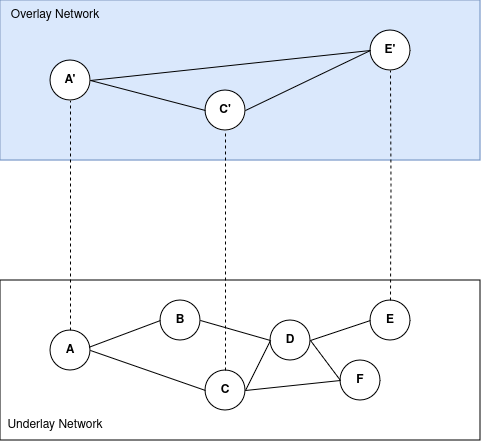
\includegraphics[width=0.5\textwidth]{overlays.png}
\caption{Concept of a very basic overlay network. Nodes A, C and E create logical links with each other, forming an overlay network}
\label{fig:overlay}
\end{figure}

\subsection{Security in Overlay Networks}

The Internet is built on public infrastructure users generally have no control over. Public routers, relay nodes, servers and even physical links always carry the risk of traffic eavesdropping and tampering by untrusted entities. Although overlay networks are able to create a logical communication structure, traffic can still be routed through this susceptible infrastructure before reaching its destination node. Therefore, to ensure the confidentiality, privacy and integrity of connections established through an insecure medium, data should be properly encrypted and authenticated.

In fact, if the Internet application running in the nodes of an overlay network has no such security considerations, communication will always be subjected to network attack vectors such as \ac{mitm} and \ac{dos} attacks and traffic snooping.

To add a confidentiality layer to communication, overlay networks employ security mechanisms which encapsulate datagrams, ensuring only designated overlay nodes can interpret the transmitted information. A common way to achieve this functionality is the use of \acp{vpn}.

\subsection{Virtual Private Networks}

Conceptually, a \ac{vpn} is a virtual network that provides functionalities  securing the transmission of data between any two endpoints ~\cite{HARMENING2017843}. \acp{vpn} have been a widely used technology for decades, establishing itself as the backbone to secure communications over the Internet.

The following sections aim to analyse how \ac{vpn} services have evolved, from its traditional design to more recent paradigms, which are able to tackle complexity and scalability issues. Then, it presents an individual overview of notable \ac{vpn} providers and compares their respective advantages, limitations, trade-offs and suitability for the scope of this solution. This state of the art technological survey aims to pickup on similar works ~\cite{zuqueteseguranca, berger2006analysis}, which examine established protocols such as OpenVPN and IPSec, while additionally reviewing modern protocols, focusing on WireGuard. This exploration serves as the foundation for understanding which protocol is the most suitable to secure communications for the scenario at hand.


\iffalse
\subsubsection{VPN Toplogies}

Not all \ac{vpn} providers have the same structural design. In fact, even individual \ac{vpn} services can be deployed to suit different use cases. Grasping the architectural capabilities and limitations of popular \ac{vpn} topologies is fundamental to evaluate the suitability of a service for a given scenario. Therefore, before individually analysing \ac{vpn} providers, this section presents a review on the advantages, disadvantages and applications of the most common \ac{vpn} topologies.

Traditional \ac{vpn} services operate under a \textbf{hub-and-spoke} architecture, a model composed by one or more \ac{vpn} Gateways - devices accepting incoming connections from client nodes and forwarding the traffic to their final destination. Hub-and-spoke architectures carry some well known bottlenecks ~\cite{ELHEDHLI20051615, o1998geographer} and, more recently, ~\cite{AN2015103}. First, it implies increased latency associated with the geographical distance between a client and the nearest hub. This topology also raises reliability issues as hubs introduce a single point of failure to the system, requiring backup plans and alternative routes to ensure no network down times.

To avoid the congestion associated with hub-and-spoke architectures, decentralized topologies have emerged which operate by establishing direct \ac{p2p} connection between clients, creating a mesh network.
\fi

\subsubsection{VPNs on NAT Networks}
\label{ss:nat-t}

A \ac{nat} is a networking mechanism responsible for translating \ac{ip} addresses in private networks to public addresses when packets sent from a private network are routed to the public Internet. In the context of \ac{vpn} communications, this process can prove to be a major constraint, not only due to \ac{nat}'s tampering of \ac{ip} packets' fields, namely destination and source addresses, which could potentially compromise its integrity in the eyes of a \ac{vpn} protocol, but also regarding the dynamically changing public \ac{ip} addresses which \ac{nat} decides to translate private addresses to. In other words, without additional tools, a host in a private network has no knowledge regarding which public \ac{ip} it will be assigned.

In fact, it is very likely that devices connected to the Internet reside in a network behind both \ac{nat} mechanisms and Firewall rules, with no open ports. Also, believing nodes will have a consistent static \ac{ip} is a very naive assumption, especially when considering mobile devices. NAT Traversal is a networking technique that enables the establishing and maintaining (by keeping \ac{nat} holes open) of \ac{p2p} connections between two peers, no matter what's standing between them, making communication possible without the need for firewall configurations or public-facing open ports. There's no one solution to achieve this functionality. In fact, there are various developments effectively implementing a NAT Traversal solution, such as ICE ~\cite{rfc8445} and STUN ~\cite{rfc8489}. Hence, each \ac{vpn} service can have its own way of supporting NAT Traversal. Each case is explored separately.


\section{VPN Providers}

\subsection{IPSec}

IPSec refers to an aggregation of layer 3 protocols that work together to create a security extension to the \ac{ip} protocol by adding packet encryption and authentication. Conceptually, IPSec presents two main dimensions: the protocol defining the transmitted packets' format, when security mechanisms are applied to them, and the protocol defining how parties in a communication negotiate encryption parameters.

Communication in an IPSec connection is managed according to \acp{sa}. A \ac{sa} is an unidirectional set of rules and parameters specifying the necessary information for secure communication to take place ~\cite{rfc4301}. Here, unidirectional means a \ac{sa} can only be associated with either inbound or outbound traffic, but never with both. Hence, an IPSec bidirectional association implies the establishment of two \acp{sa}: one for incoming packets and one for outgoing. \acp{sa} specify which security mechanism to use - either \ac{ah} or \ac{esp} - and are identified by a numeric value, the \ac{spi}. Although \ac{sa}s can be manually installed in routers, gateways or machines, it becomes impractical as more clients appear. \ac{ike} ~\cite{rfc7296} is a negotiation protocol that tackles the problems associated with manual \ac{sa} installation. In fact, \ac{ike} allows the negotiation of \ac{sa} pairs between any two machines through the use of asymmetric keys or shared secrets.

\subsubsection{Transport and Tunnel modes}

IPSec supports two distinct modes of functionality: transport and tunnel ~\cite{rfc4301}, which differ in the way traffic is dealt with and processed. In the context of \acp{vpn}, tunnel mode presents the
most desirable characteristics. First, tunnel mode encapsulates the original \ac{ip} packet, allowing the use of private \ac{ip} addresses as source or destination. Tunnel mode creates the concept of an ``outer" and ``inner`` \ac{ip} header. The former contains the addresses of the IPSec peers, while the latter contains the real source and destination addresses. Moreover, this very same encapsulation adds confidentiality to the original addresses.

Transport mode requires fewer computational resources and, consequently, carries less protocol overhead. It does not, however, provide much security compared to tunnel mode, so, to secure data in a communication, tunnel mode's total protection and confidentiality of the encapsulated \ac{ip} packet carry much more valuable functionalities.

\subsubsection{Authentication Header}

\ac{ah} is a protocol in the IPSec suite providing data origin validation and data integrity consisting in the generation of a checksum via a digest algorithm ~\cite{rfc4302}. Additionally, besides the actual message under integrity check, two other parameters are used under the \ac{ah} mechanism. First, to ensure the message was sent from a valid origin, \ac{ah} includes a secret shared key. Then, to ensure replay protection, it also includes a sequence number. This last feature is achieved with the sender incrementing a sequence integer whenever an outgoing message is processed.

\ac{ah}, as the name suggests, operates by attaching a header to the \ac{ip} packets, containing the message's \ac{spi}, its sequence number, and the \ac{icv} value. This last field is then verified by receivers, which calculate the packet's \ac{icv} on their end. The packet is only considered valid if there's a match between the sender and receiver's \ac{icv}.

Where this header is inserted depends on the mode in which IPSec is running. In transport mode, the \ac{ah} appears after the \ac{ip} header and before any next layer protocol or other IPSec headers. As for tunnel mode, the \ac{ah} is injected right after the outer \ac{ip} header.

To calculate the \ac{icv}, the \ac{ah} requires the value of the source and destination addresses, which raises an incompatibility when faced with networks operating with \ac{nat} mechanisms ~\cite{frankel2005guide}.

\subsubsection{Encapsulating Security Payload}

The \ac{esp} protocol also offers authentication, integrity and replay protection mechanisms. It differs from \ac{ah} by also providing encryption functionalities, where peers in a communication use a shared key for cryptographic operations. Analogous to the previous protocol, the \ac{esp}'s header location differs in different IPSec modes. In transport mode, the header is inserted right after the \ac{ip} header of the original packet. Also, in this mode, since the original \ac{ip} header is not encrypted, endpoint addresses are visible and might be exposed. As for tunnel mode, a new \ac{ip} header is created, followed by the \ac{esp} header.

Tunnel mode \ac{esp} is the most commonly used IPSec mode. This setup not only offers original \ac{ip} address encryption, concealing source and destination addresses, but also supports the addition of padding to packets, hampering cipher analysis techniques. Moreover, it can be made compatible with \ac{nat} and employ \ac{nat}-traversal techniques ~\cite{nam2022high, singh2012nat}.

\subsection{OpenVPN}

OpenVPN ~\cite{ovpnwebsite} is yet another open-source \ac{vpn} provider, known for its portability among the most common operating systems due to its user-space implementation. OpenVPN uses established technologies, such as \ac{ssl} and asymmetric keys for negotiation and authentication and IPSec's \ac{esp} protocol, explored in the previous section, over UDP or TCP for data encryption.

\subsubsection{TUN and TAP interfaces}

OpenVPN's virtual interfaces, which process outgoing and incoming packets, have two distinct types: TUN (short for internet TUNnel) and TAP (short for internet TAP). Both devices work quite similarly, as both simulate \ac{p2p} communications. They differ on the level of operation, as TAP operates at the Ethernet level. In short, TUN allows the instantiation of \ac{ip} tunnels, while TAP instantiates Ethernet tunnels.

\subsubsection{OpenVPN flow}

When a client sends a packet through a TUN interface, it gets redirected to a local OpenVPN server. Here, the server performs an \ac{esp} transformation and routes the \ac{ip} packet to the destination address, through the ``real" network interfaces.

Similarly, when receiving a packet, the OpenVPN server will perform decipherment and validation operations on it, and, if the \ac{ip} packet proves to be valid, it is sent to the TUN interface.

This process is analogous when dealing with TAP devices, differing, as mentioned before, at the protocol level.

\subsection{WireGuard}
\label{ss:wg}

WireGuard ~\cite{donenfeld2017wireguard} is an open-source \ac{udp}-only layer 3 network tunnel implemented as a kernel virtual network interface. WireGuard offers both a robust cryptographic suite and transparent session management, based on the fundamental principle of secure tunnels: peers in a WireGuard communication are registered as an association between a public key (analogous to the OpenSSH keys mechanism) and a tunnel source \ac{ip} address.

One of WireGuard's selling points is its simplicity. In fact, compared to similar protocols, which generally support a wide range of cryptographic suites, WireGuard settles for a singular one. Although one may consider the lack of cipher agility as a disadvantage, this approach minimizes protocol complexity and increases security robustness by avoiding vulnerabilities commonly originating from such protocol negotiation ~\cite{curguz2016vulnerabilities}.

\subsubsection{Routing}

Peers in a WireGuard communication maintain a data structure containing their own identification (both public and private keys) and interface listening port. Then, for each known peer, an entry is present containing an association between a public key and a list of allowed source \ac{ip}s.

This structure is queried on communication initiation. When a peer wants to start a connection, the structure is consulted, and, based on the destination address, the destination peer's public key is retrieved to ecnrypt an initial handshake message for session key exchange. As for data exchanging, after encryption operations (using the session keys), the structure is used to verify the validity of the packet's source address, which, in other words, means checking if there's a match between the source address and the allowed addresses present on the routing structure for that peer.

Optionally, WireGuard peers can configure one additional field, an internet endpoint, defining the listening address where packets should be sent. If not defined, the incoming packet's source address is used.

\subsubsection{Cipher Suite}

As mentioned before, WireGuard offers a single cipher suite for encryption and authentication mechanisms in its protocol. The peers' pre-shared keys are Curve25519 points, an implementation of an elliptic-curve-Diffie-Hellman function, characterized by its strong conjectured security level - presenting the same security standards as other algorithms in public key cryptography - while achieving record computational speeds ~\cite{bernstein2006curve25519}. Additionally, WireGuard's Curve25519 computation uses a verified implementation ~\cite{zinzindohoue2017hacl}, which contributes further to the robustness of the protocol's cryptography.

Before any encrypted data exchange actually happens, WireGuard enforces a handshake for symmetric session key exchange. The messages involved in this handshake process follow a variation of the Noise ~\cite{perrin2018noise} protocol, which is essentially a state machine controlled by a set of variables maintained by each peer in the negotiation.

Regarding payload data cryptography, a WireGuard message's data is encrypted with session keys and a nonce counter, using ChaCha20Poly1305, a Salsa20 variation ~\cite{bernstein2008chacha}. The ChaCha cryptographic family offers robust resistance to crypto-analytic methods ~\cite{cryptoeprint:2014/613}, without sacrificing its state-of-the-art performance.

\subsubsection{Security}

On top of its robust cryptographic specification, WireGuard includes in its design a set of mechanisms to further enhance protocol security and integrity.

In fact, WireGuard presents itself as a silent protocol. In other words, a WireGuard peer is essentially invisible when communication is attempted by an illegitimate party. Packets coming from an unknown source are just dropped, with no leak of information to the sender.

Additionally, a cookie system is implemented in an attempt to mitigate \ac{ddos} attacks. Since, to determine the authenticity of a handshake message, a Curve25519 multiplication must be computed, a CPU intensive operation, a CPU-exhaustion attack vector could be exploited. Cookies are introduced as a response message to handshake initiation. These cookie messages are used as a peer response when under high CPU load, which is then in turn attached to the sender's following messages, allowing the requested handshake to proceed when the overloaded peer has available resources to continue.

\subsubsection{Basic WireGuard Configuration}

Connecting two peers in a WireGuard communication can be done with minimal configuration. After the generation of an asymmetric key pair and the setup of a WireGuard interface, it is only required to add the other peer to the routing table with its public key, allowed \ac{ip}s and, optionally, its internet endpoint. After both peers configure each other, the tunnel is established and packets can be transmitted through the WireGuard interface.
In a practical scenario, given two peers, \emph{A} and \emph{B}, with pre-generated keys and internet interfaces, presented on table \ref{tab:wgconfpeers}, the CLI steps to setup a minimal WireGuard communication, as specified in the official WireGuard documentation are presented in figure \ref{fig:wgconf}.


\begin{table}[]
\centering
\begin{tabular}{c|l|l|}
\cline{2-3}
\multicolumn{1}{l|}{}                            & \multicolumn{1}{c|}{\textbf{Peer A}} & \multicolumn{1}{c|}{\textbf{Peer B}} \\ \hline
\multicolumn{1}{|c|}{\textbf{Private Key}}       & gIb/+...+uF2Y=                       & aFov...G3l0=                         \\ \hline
\multicolumn{1}{|c|}{\textbf{Public Key}}        & FeQI...jHgE=                         & sg0X...7kVA=                         \\ \hline
\multicolumn{1}{|c|}{\textbf{Internet Endpoint}} & 192.168.100.4                        & 192.168.100.5                        \\ \hline
\multicolumn{1}{|c|}{\textbf{WireGuard Port}}    & 51820                                & 51820                                \\ \hline
\end{tabular}
\caption{Nodes to be configured with a WireGuard tunnel}
\label{tab:wgconfpeers}
\end{table}

\begin{figure}
\begin{multicols}{2}
\begin{lstlisting}[language=sh, frame=single, breaklines=true, breakatwhitespace=true, basicstyle=\small]
# Peer A - interface setup
$ ip link add wg0 type WireGuard
$ ip addr add 10.0.0.1/24 dev wg0
$ wg set wg0 private-key ./private
$ ip link set wg0 up

# Adding peer B to known peers
$ wg set wg0 peer sg0X...7kVA= allowed-ips 10.0.0.2/32 endpoint 192.168.100.5:51820
$

\end{lstlisting}
\columnbreak
\begin{lstlisting}[language=sh, frame=single, breaklines=true, breakatwhitespace=true, basicstyle=\small]
# Peer B - interface setup
$ ip link add wg0 type WireGuard
$ ip addr add 10.0.0.2/24 dev wg0
$ wg set wg0 private-key ./private
$ ip link set wg0 up

# Adding peer A to known peers
$ wg set wg0 peer FeQI...jHgE= allowed-ips 10.0.0.1/32 endpoint 192.168.100.4:51820
$

\end{lstlisting}
\end{multicols}
\caption{Basic WireGuard Communication Between Two Peers}
\label{fig:wgconf}
\end{figure}

\subsubsection{Limitations}
\label{sec:wglimits}

Although WireGuard proves to be a robust, performant and maintainable protocol for encrypted communication, it still presents some complexity regarding administration agility and scalability, since it (intentionally) lacks a coordination entity. New clients added to a stand-alone WireGuard network imply the manual reconfiguration of every other peer already present, a process with added complexity and prone to errors, if carried out manually.

There are, however, several software products implementing such an orchestrator, which provide functionalities to easily manage WireGuard peers and respective tunnels, such as Tailscale, Netbird or Netmaker. These solutions are explored in further sections.

\subsection{Protocol Comparison}

\subsubsection{Security}

Regarding security, although all analysed providers are capable of robustly authenticating and encrypting data, recent verifications of WireGuard's cryptographic suite \cite{lipp2019mechanised, dowling2018cryptographic} conclude WireGuard offers a smaller attack surface, when compared with OpenVPN and IPSec.

\subsubsection{Performance}

The concept of performance in \ac{vpn} applications refers to the impact the protocol has on communications. This dimension can be empirically measured, by analysing metrics like \ac{rtt}, throughput and jitter. CPU utilization is also a valuable metric, as demanding operations can also take a toll on overall network performance, since processing traffic might stall due to the CPU overloading.

The performance claims on ~\cite{donenfeld2017wireguard}, which compares WireGuard to other discussed technologies, present results in favour of WireGuard in such performance tests. This conclusion is backed by more extensive research ~\cite{mackey2020performance, osswald2020performance}, where communication is tested in a wide range of different network scenarios and CPU architectures.

WireGuard's kernel implementation and efficient multi-threading usage contribute greatly to such performance benchmarks. Overall, WireGuard outperforms IPSec and OpenVPN with no notable trade-offs.

\subsubsection{Usability}

Usability in \ac{vpn} protocols refers to the ease of use regarding service configuration and management. IPSec's configuration can be quite complex, due to its cryptographic directives and protocol negotiation. Also, the several different modes IPSec can be configured to run in might prove overwhelming for unfamiliar users. OpenVPN's GUI provides a user-friendly platform to easily administrate the software, still requiring, however, a considerable degree of technical expertise. WireGuard, however, is able to combine protocol simplicity, as it enforces a single cipher suite, with straightforward configuration directives. In fact, as we've seen in Section \ref{ss:wg}, configuring WireGuard peers requires no knowledge of the protocol's specification.

Table \ref{tab:protocomp} summarizes the above analysis.


\begin{table}[]
\centering
\resizebox{\textwidth}{!}{%
\begin{tabular}{c|c|c|c|}
\cline{2-4}
                                             & \textbf{IPSec}                    & \textbf{OpenVPN}                                                                          & \textbf{WireGuard}                    \\ \hline
\multicolumn{1}{|c|}{\textbf{Security}}      & Robust, but complex               & \begin{tabular}[c]{@{}c@{}}Generally robust,\\ requires proper configuration\end{tabular} & Modern, recently verified cryptography \\ \hline
\multicolumn{1}{|c|}{\textbf{Usability}}     & Requires expertise                & Requires expertise                                                                        & Minimal configuration                 \\ \hline
\multicolumn{1}{|c|}{\textbf{Performance}}   & \begin{tabular}[c]{@{}c@{}}Good, but underperforms \\ compared to WireGuard \end{tabular}                         & Generally implies higher latencies                                                        & Overall, outperforms other protocols  \\ \hline
\multicolumn{1}{|l|}{\textbf{NAT-Traversal}} & Supported, requires configuration & Supported, requires configuration                                                         & Seamless integration                  \\ \hline
\end{tabular}%
}
\caption{VPN protocol's performance and features comparison}
\label{tab:protocomp}
\end{table}


\subsection{Summary}

This section presents the fundamentals of \acp{vpn} and how they are able to ensure integrity and confidentiality to communication through insecure mediums. Then, some of the most notable \ac{vpn} providers were reviewed and compared, regarding functionalities and overall performance. The result of this analysis suggests WireGuard as the most promising \ac{vpn} protocol, due to its ease of management and configuration, security mechanisms and verified cryptography.


\section{WireGuard Coordination}
\label{sec:coordination}

In Section \ref{sec:wglimits}, the lack of a coordination entity on stand-alone WireGuard topologies was raised as a possible limitation. In fact, manually reconfiguring peers in a standalone WireGuard network is a process that scales terribly. Moreover, on highly restrictive networks, creating direct WireGuard tunnels proves to not be as straightforward.

With such constraints in mind, this section explores applications and implementations of coordination platforms built, or with the potential to be built, on top of WireGuard, aiming to create a seamless peer orchestration and configuration process, minimizing human intervention.

\subsection{Tailscale}

Tailscale ~\cite{tailscale2020online} is a \ac{vpn} service operating with a Golang user-space WireGuard variant as its data plane. Tailscale operates under a hybrid \ac{vpn} model. Although a central entity is present, initially resembling hub-and-spoke topologies, its main purpose is to aid clients in configuring themselves and managing connections, serving nearly no traffic.

In addition to orchestrating the configuration and establishment of WireGuard tunnels, Tailscale also employs a set of mechanisms capable of addressing network constraints which would hinder the process of directly creating WireGuard connections. In fact, Tailscale praises itself as being able to make any two clients communicate, regardless of the network structure and security policies standing in-between them. For the scope of this project, where very few is known about \ac{ua}'s network architecture, the ability to bypass such constraints would prove extremely valuable.

This section explores how Tailscale is able to manage the WireGuard links between its clients, creating a WireGuard encrypted overlay network while dealing with security constraints preventing such communications to take place.

\subsubsection{Architecture}

Tailscale's central entity, referred to as the \textbf{coordination server}, functions as a shared repository of peer information, used by clients to retrieve data regarding other nodes and establish on-demand WireGuard connections among each other.

This approach differs from traditional hub-and-spoke since the coordination server carries nearly no traffic, it only serves encryption keys and peer information. Tailscale's architecture provides the best of both worlds, benefiting from the advantages of a centralized entity facilitating dynamic reconfigurations and peer discovery without bottlenecking WireGuard's data exchanging performance.

In practical terms, a Tailscale client will store, in the coordination server, its own public key and where it can currently be found. Then, it downloads a list of public keys and addresses that have been stored on the server previously by other clients. With this information, the client node is able to configure its Tailscale interface and establish direct communications with any other node in its domain.

\subsubsection{Overcoming restrictive networks}
\label{ssec:tsnetworks}

There are, however, some network security configurations which prevent WireGuard tunnels from being established. For example, firewalls blocking \ac{udp} traffic entirely prevent the creation of direct WireGuard tunnels between two peers. In addition to orchestrating WireGuard peers, Tailscale is also able to overcome such constrained networks.

Regarding stateful firewalls, where, generally, inbound traffic for a given source address on a non-open port is only accepted if the firewall has recently seen an outgoing packet with such \emph{ip:port} as destination, Tailscale keeps, in its coordination server, the public address of each node in its network. With this information, if both peers send an outgoing packet to each other at approximately the same time (a time delta inferior to the firewall's cache expiration), then the firewalls at each end will be expecting the reception of packets from the opposite peer. Hence, packets can flow bidirectionally and a \ac{p2p} communication is established. To ensure this synchronism of attempting communication at approximate times, Tailscale uses its coordination server and \ac{DERP} servers (explored further in the following paragraphs) as a side channel.

Although this procedure is quite effective, in networks with \ac{nat} mechanisms, where source and destination addresses are tampered with, this process is not as straightforward, since peers don't know the public addresses \ac{nat} will translate their private addresses to. The \ac{stun} protocol offers aid in performing \ac{nat}-Traversal operations ~\cite{rfc8489} and its supported by Tailscale to overcome this problem. For a peer to discover and store in the coordination server its own public \emph{ip:port}, it first sends a \ac{udp} message requesting an \ac{ip} binding to a \ac{stun} server. Upon receiving this request, the \ac{stun} server, which can see the public source address of the packet it received, or, by other words, the address produced by \ac{nat}, replies this value to the peer.

There are, however, some \ac{nat} devices that create a completely different public address mapping for each different destination a machine communicates with, which hinders the above address discovery process, since the address the \ac{stun} server sees might not match when communicating with a different destination. Such \ac{nat} devices are classified as \ac{edm} (in opposition to \ac{eim}) ~\cite{rfc4787}.

Networks employing \ac{edm} \ac{nat} devices and/or really strict firewall rules, render these traversal techniques useless. To enable \ac{p2p} communications in such scenarios, Tailscale also provides a network of \ac{DERP} servers, which are responsible for relaying packets over \ac{http}. A Tailscale client is able to forward its encrypted packets to one of such \ac{DERP} servers. Since a client's private key never actually leaves its node, \ac{DERP} servers can't decrypt the traffic being relayed, performing only redirection of already encrypted data. Tailscale offers a geographically distributed fleet of such servers. However, since traffic is encapsulated as an \ac{http} stream, relayed communications always imply a degradation of network performance.

Hence, Tailscale connections can be of two types: either \textbf{direct} or \textbf{relayed}. Tailscale will always attempt to create direct connections. In fact, if \ac{nat}-traversal succeeds on both endpoints and there are no restrictions to \ac{udp} traffic, a direct WireGuard tunnel can be established. However, on networks employing \ac{edm} \ac{nat} mappings and/or \ac{udp} blocking firewalls, direct connections cannot be formed. That's where relayed connections are created. Clients on relayed connections encapsulate WireGuard \ac{udp} packets as \ac{tcp} streams and forwards them through \ac{http} to the closest \ac{DERP} server available, which in turn delivers them to its destination.

\subsubsection{Headscale}
\label{sec:hs}

While Tailscale's client is open source, its coordination server isn't. There is, however, an open-source, self-hosted alternative to Tailscale's control server, Headscale. Headscale ~\cite{headscale2023online} provides a narrow-scope implementation (with a single Tailscale private network) of the aforementioned coordination server, which, in the authors' words, is mostly suitable for personal use and small organizations. Nodes running Tailscale clients can opt to specify the location of the control server, which can be the address of a running self-hosted Headscale instance.

Headscale also supports the self-hosting of \ac{DERP} and \ac{stun} servers. This is useful as it allows the self-hosting of a complete Tailscale solution.

\section{University of Aveiro Network}
\label{sec:uanet}

Due to security and privacy concerns, the specification of \ac{ua}'s network topology is not publicly available nor is it made available for this dissertation. As such, it is perceived as a black box. There are, however, a few reachable conclusions drawn from observing its behaviour.

In fact, \ac{ua}'s network is highly segmented, where clients are grouped according to their roles. When clients connect to an \ac{ap} within the campus, they are connected to a \ac{vlan} shared by several other clients, in which the private resources are accessible. Regarding \ac{nat}, the present mechanisms in the network are unknown, as are their mappings' \ac{ttl}, which is an important variable mentioned in Section \ref{ssec:tsnetworks} to perform \ac{nat}-traversal techniques.

Any other specification of \ac{ua}'s network is unknown. Moreover, the network's firewall rules can't be altered to suit our needs.

\section{Robot Operating System}

\ac{ros} \footnote{https:www.ros.org/} is an open-source meta-operating system which provides an ecosystem for the development and distribution of robot software. \ac{ros} is considered a meta-operating system as it operates alongside a standard operating system, introducing a virtualization layer between applications and computational resources ~\cite{pyo_ros_en_2017}. In other words, \ac{ros} abstracts developers from the hardware specification the applications will run on. Hence, \ac{ros} applications can be ported and reused across multiple devices, without requiring additional hardware-specific configurations or implementations. Moreover, communication through \ac{ros} is possible when dealing with devices employing distinct hardware implementations.

At its core, \ac{ros} is a combination of hardware abstraction operations, intra-process communication, device controllers and package management. Additionally, \ac{ros} includes a set of applications which implement common desired robot functionalities, such as navigation and object recognition. Due to its design focused on reusability and modularity, \ac{ros} packages developed by the community can easily be integrated in new applications.    

\subsection{\ac{ros} Master-Slave model}

Any \ac{ros} application is composed of one or more nodes. A \ac{ros} node is perceived as the most basic program execution unit, generally serving a specific single purpose in order to optimize reusability. A \ac{ros} application also implies the existence of a master node, responsible for providing other nodes (called slaves) with on-demand information regarding each other. Slave nodes store their information in the master node and retrieve information regarding other slaves when necessary. Hence, a \ac{ros} master will act as a disocvery server, allowing nodes to learn the services running in other application peers and the addresses they should request connections to in order to use them. Communication between a master and its slaves is done using the \ac{xmlrpc} protocol, a lightweight \ac{http} based protocol.       

\subsection{Messages}

Nodes in a \ac{ros} application exchange data through messages. A \ac{ros} message is essentially a set of fields, each defined by a data type and value pair. Message fields can be defined as basic data types, arrays or even nest other messages. Messages are serialized and trasmitted using variations of \ac{tcp} and \ac{udp}. 

\subsection{Communication}

Having described how nodes in a \ac{ros} application discover themselves and how data is represented, the following paragraphs overview three distinct communication scenarios. For asynchronous communication, useful for data streams such as infromation captured by sensors, \ac{ros} supports a topic based publish-subscribe channel. In these communications, nodes can act as either publisher or subscribers. Publisher nodes, after registering their information and topic in the master, are responsible for pushing messages associated with such topic, delivering them to registered subscriber nodes. Subscriber nodes interested in a topic query the master node for the addresses of publishers registered under that topic. Then, to consume the information, a subscriber node establishes a direct connection with a publisher, where the message stream is made available.

In scenarios where a request-response communication is more suitable, \ac{ros} implements a mechanism refered to as services, which operate as a classic client-server model. In fact, a \ac{ros} service implies the existence of a server node, which listens and handles client node requests. As a synchronous communication, clients are able to perform requests to such a node server and receive its result as a response. Both request and response are defined as \ac{ros} messages, previously explored.

Finally, \ac{ros} introduces the concept of actions. Actions can be perceived as an extension of services, suitable for long running tasks where feedback about operation status is required. Similarly to services, a client will request an action server to execute a set of tasks. However, instead of solely responding with the output for a given requests, action servers are able to report to clients the status of the procedure. Moreover, clients can issue an action cancel to a server, which aborts the server's action entirely.

\chapter{Proposed Overlay Network Manager}

Having outlined the relevant research, background and technologies for this dissertation's scope, this chapter details the development of a WireGuard based overlay network manager.

\section{Architecture}

The solution's main goal is to create a communication protocol capable of establishing a link between two clients residing behind a network with firewall rules preventing direct connections from taking place. To connect peers in such a scenario, the solution introduces a relay server in the network, reachable to any client, which acts as an intermediary responsible for receiving and forwarding traffic from a source to a destination client. In order to ensure clients are able to communicate with such a relay, traffic is encapsulated as \ac{http}, with the server listening on a configured open port. Additionally, for the relay server to deliver a message to a destination client, nodes establish and maintain a connection with this server, bypassing the established only firewall policy, since a connection is already open and traffic can flow bidirectionally. \ac{http} is used for encapsulation since it further ensures packets get through the network's firewalls. In fact, \ac{http} is such a standard and essential protocol that it is almost always allowed through any firewall. Moreover, keeping an open channel between the clients and the relay server proves to be simpler and more manageable when using \ac{http}, namely due to the protocol's design to handle persistence and keep-alive functionalities.

Figure \ref{fig:absprob} presents the initial scenario. Both clients, while connected to the network, are unable to communicate since the firewalls at each endpoint only allow incoming traffic from already established connections.

\begin{figure}[h]
\centering
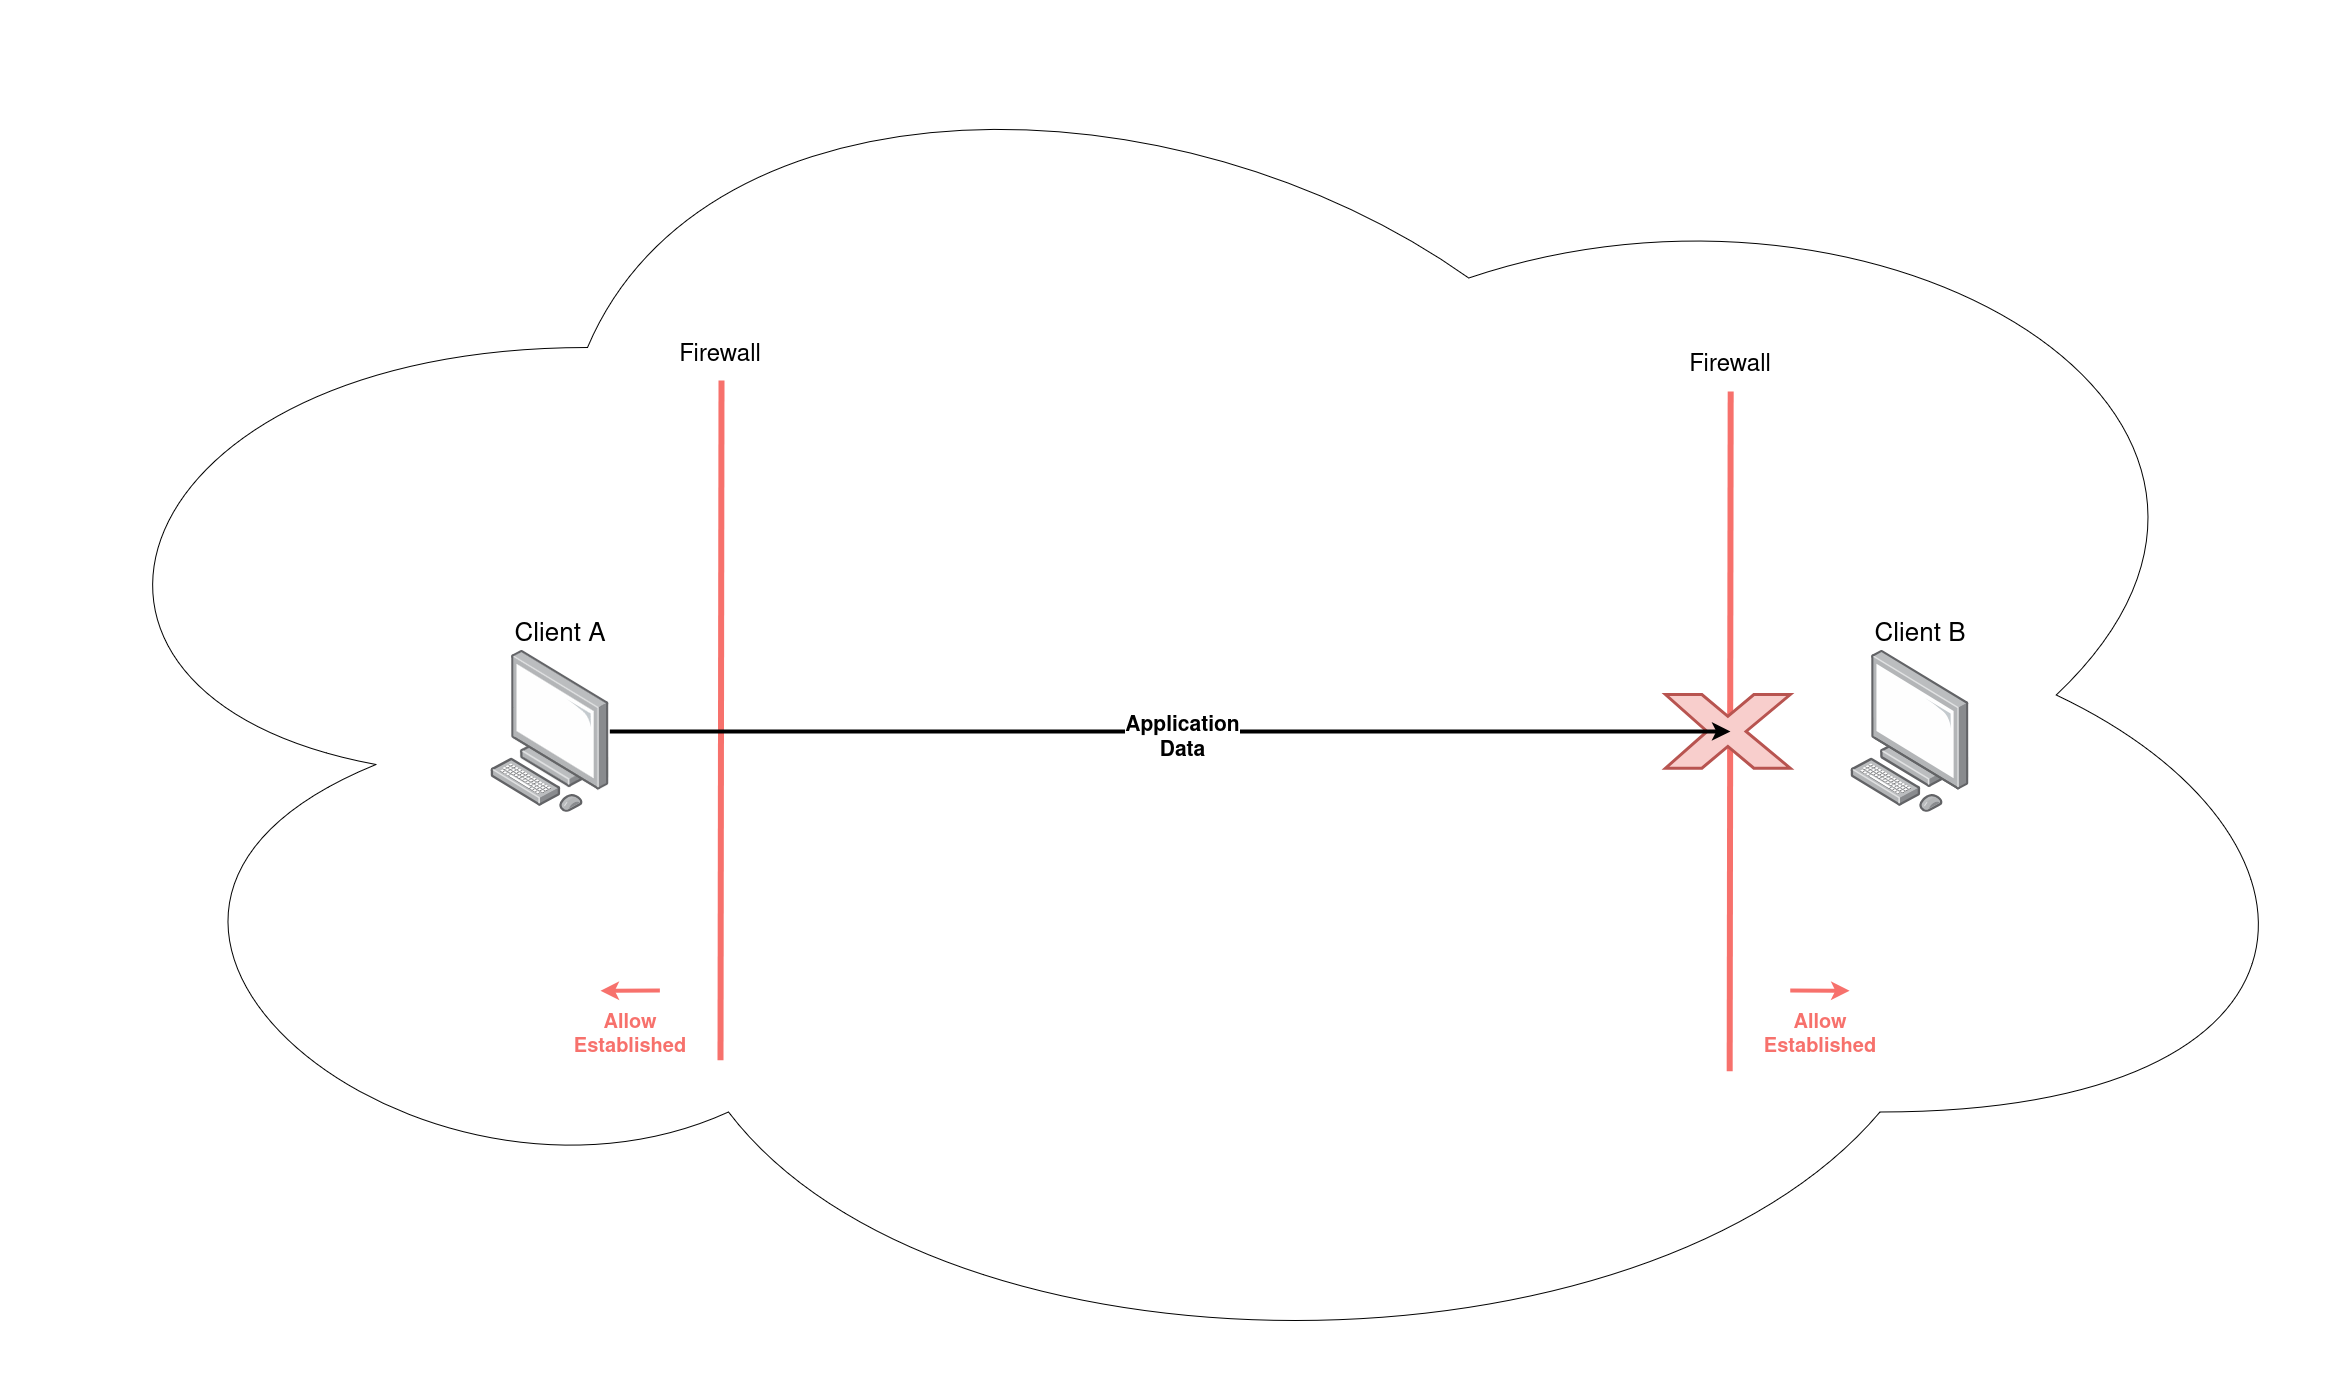
\includegraphics[width=1\textwidth]{abstract-prob.png}
\caption{Clients are unable to establish any communication due to firewall policies.}
\label{fig:absprob}
\end{figure}

In Figure \ref{fig:absrelay}, the same scenario is presented with the relay server as an intermediary. Here, both clients establish and maintain an open \ac{http} connection with the server. Using these channels, clients transmit encapsulated \ac{http} messages containing information about the destination node, which the relay server forwards through the destination client's already open connection.

\begin{figure}[h]
\centering
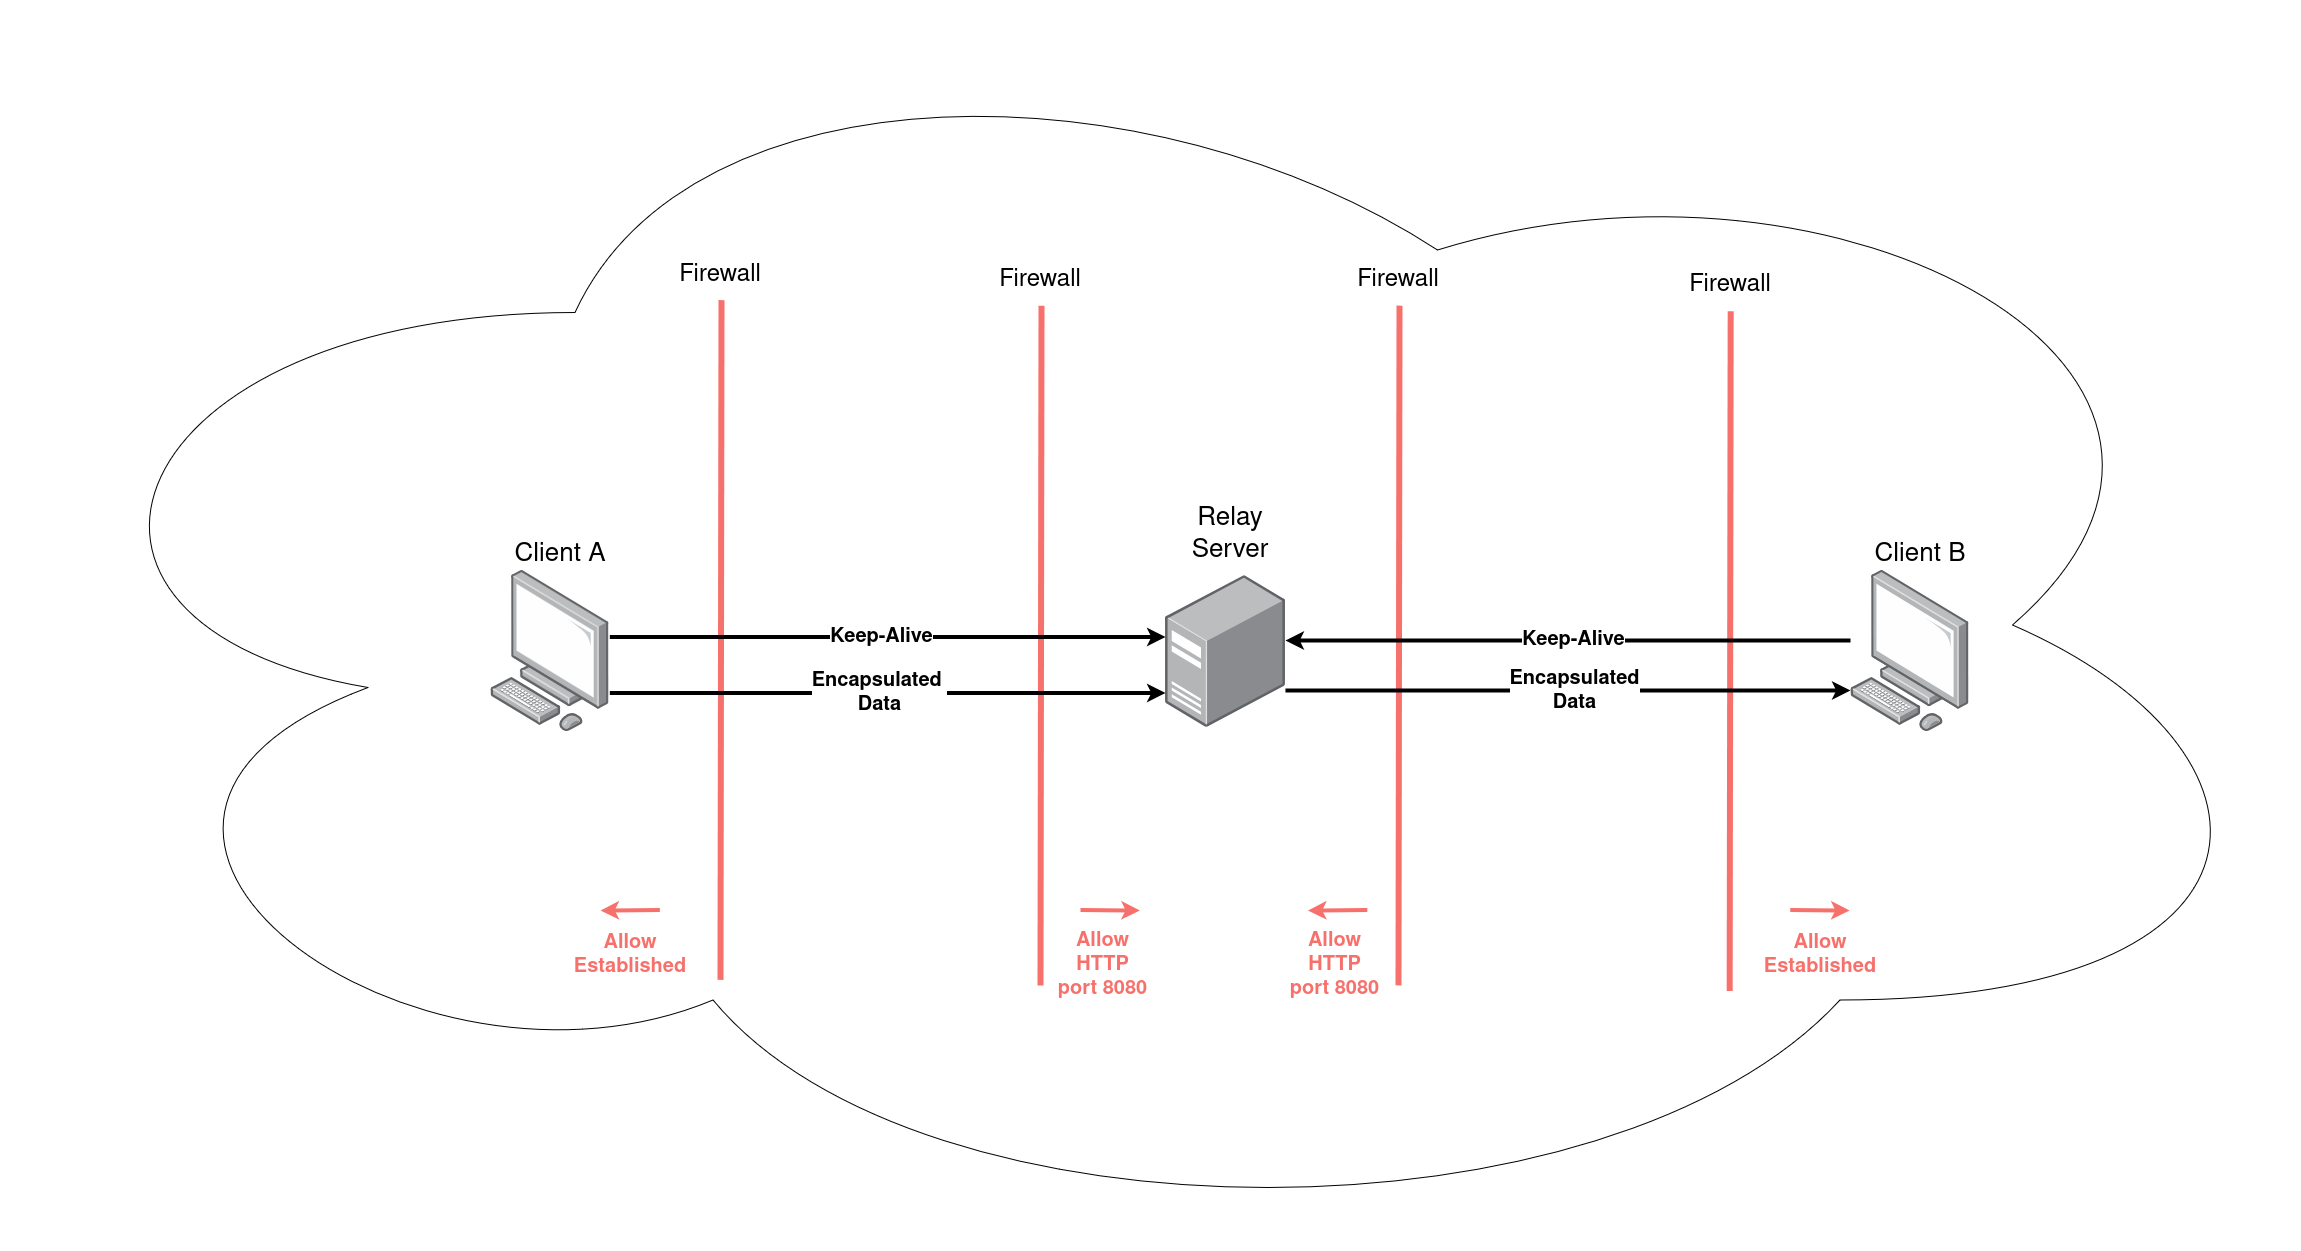
\includegraphics[width=1\textwidth]{abstract-relay.png}
\caption{Clients establish communication by forwarding traffic as HTTP to a dedicated relay server.}
\label{fig:absrelay}
\end{figure}

\section{Proposed Solution}

In Section \ref{sec:coordination}, Tailscale was explored as a WireGuard orchestrator, providing a coordination server and additional mechanisms to overcome restrictive network policies, namely \ac{udp} blocking firewalls and dynamic \ac{nat}s. We've also seen that, when Tailscale fails to establish a direct connection, a relayed channel is established instead. In fact, relayed connections operate very similarly to the outlined architecture in \ref{fig:absrelay}. Using a fleet of geographically distributed relay servers, refered to by Tailscale as \ac{DERP} servers, clients are able to encapsulate their WireGuard \ac{udp} traffic as \ac{http} and transmit it to a relay, which then delivers packets to the destination node. While both Tailscale's official coordination server and \ac{DERP} fleet could be used, this solution aims to be entirely hosted within \ac{ua}'s premises. Therefore, Headscale, covered in Section \ref{sec:hs}, is used as an alternative to Tailscale's coordination server. Regarding the relay servers, Tailscale's \ac{DERP} fleet is also discarded due to poor performance associated with geographic distance and the need for traffic confinement within \ac{ua}'s premises, again opting for a self-hosted alternative. The need for using our own \ac{DERP} is further clarified in Section \ref{ssec:hs}.

Hence, an overlay network in this solution is defined by a group of Tailscale clients, orchestrated by a self-hosted Headscale coordination server, where peers establish encrypted \ac{p2p} communications with each other through the tunnel interfaces. Tailscale's coordination server uses additional infrastructure, also self-hosted in this solution. Regarding relayed connections, Tailscale uses \ac{DERP} servers for traffic forwarding. Moreover, when dealing with direct connections, for peers to perform \ac{nat}-Traversal, required for the discovery process of their respective public addresses, Tailscale uses publicly available \ac{stun} servers. Fortunately, Headscale supports the deployment and seamless integration of both these services, allowing the self-hosting of a complete Tailscale solution within \ac{ua}'s premises.

In the University of Aveiro, where the network employs such constraints preventing clients from directly establishing \ac{p2p} connections with each other, a Tailscale peer is able to transmit its WireGuard encrypted \ac{udp} data to any other peer in its group by encapsulating packets as a \ac{tcp} stream and forwarding them over \ac{http} to a relay server. In \ac{iris}'s use case, a team of autonomous robots is configured as a group of Tailscale clients, which maintain open connections to the relay server. This allows secure \ac{p2p} communications to take place from any point in the university's campus. Additionally, developers can use their personal machines to join an overlay network and interact directly with the robots, a process which couldn't otherwise be achieved outside \ac{iris}'s network. Figure \ref{fig:absarch} depicts both this solution's architecture and the communication channels established according to distinct scenarios.

In fact, When a connection is established between two overlay peers, three different scenarios can arise, depending on the networks both source and destination nodes are communicating from. When both clients communicate from \ac{iris}'s internal network, since incoming \ac{udp} traffic is allowed and \ac{nat}-Traversal is done through the \ac{stun} endpoint listening on the coordination server, a direct Tailscale communication can take place. With one client connected to \ac{ua}'s network and one connected to \ac{iris}'s network, as the university's security policies only allow traffic from already open channels, direct WireGuard connections cannot be established. Hence, a relayed connection takes place. To communicate, clients send their packets to a relay server encapsulated as \ac{http}, which forwards the encrypted message to its destination using the previously open and persisted \ac{http} connections. To discover the address of available relays, the coordination server advertises the addresses of relay endpoints to the overlay clients. Finally, when both clients are connected to \ac{ua}'s network, the constraints are present on the two communications ends, establishing a relayed connection behaving exactly in the same way as the previous scenario.

\begin{figure}[h]
\centering
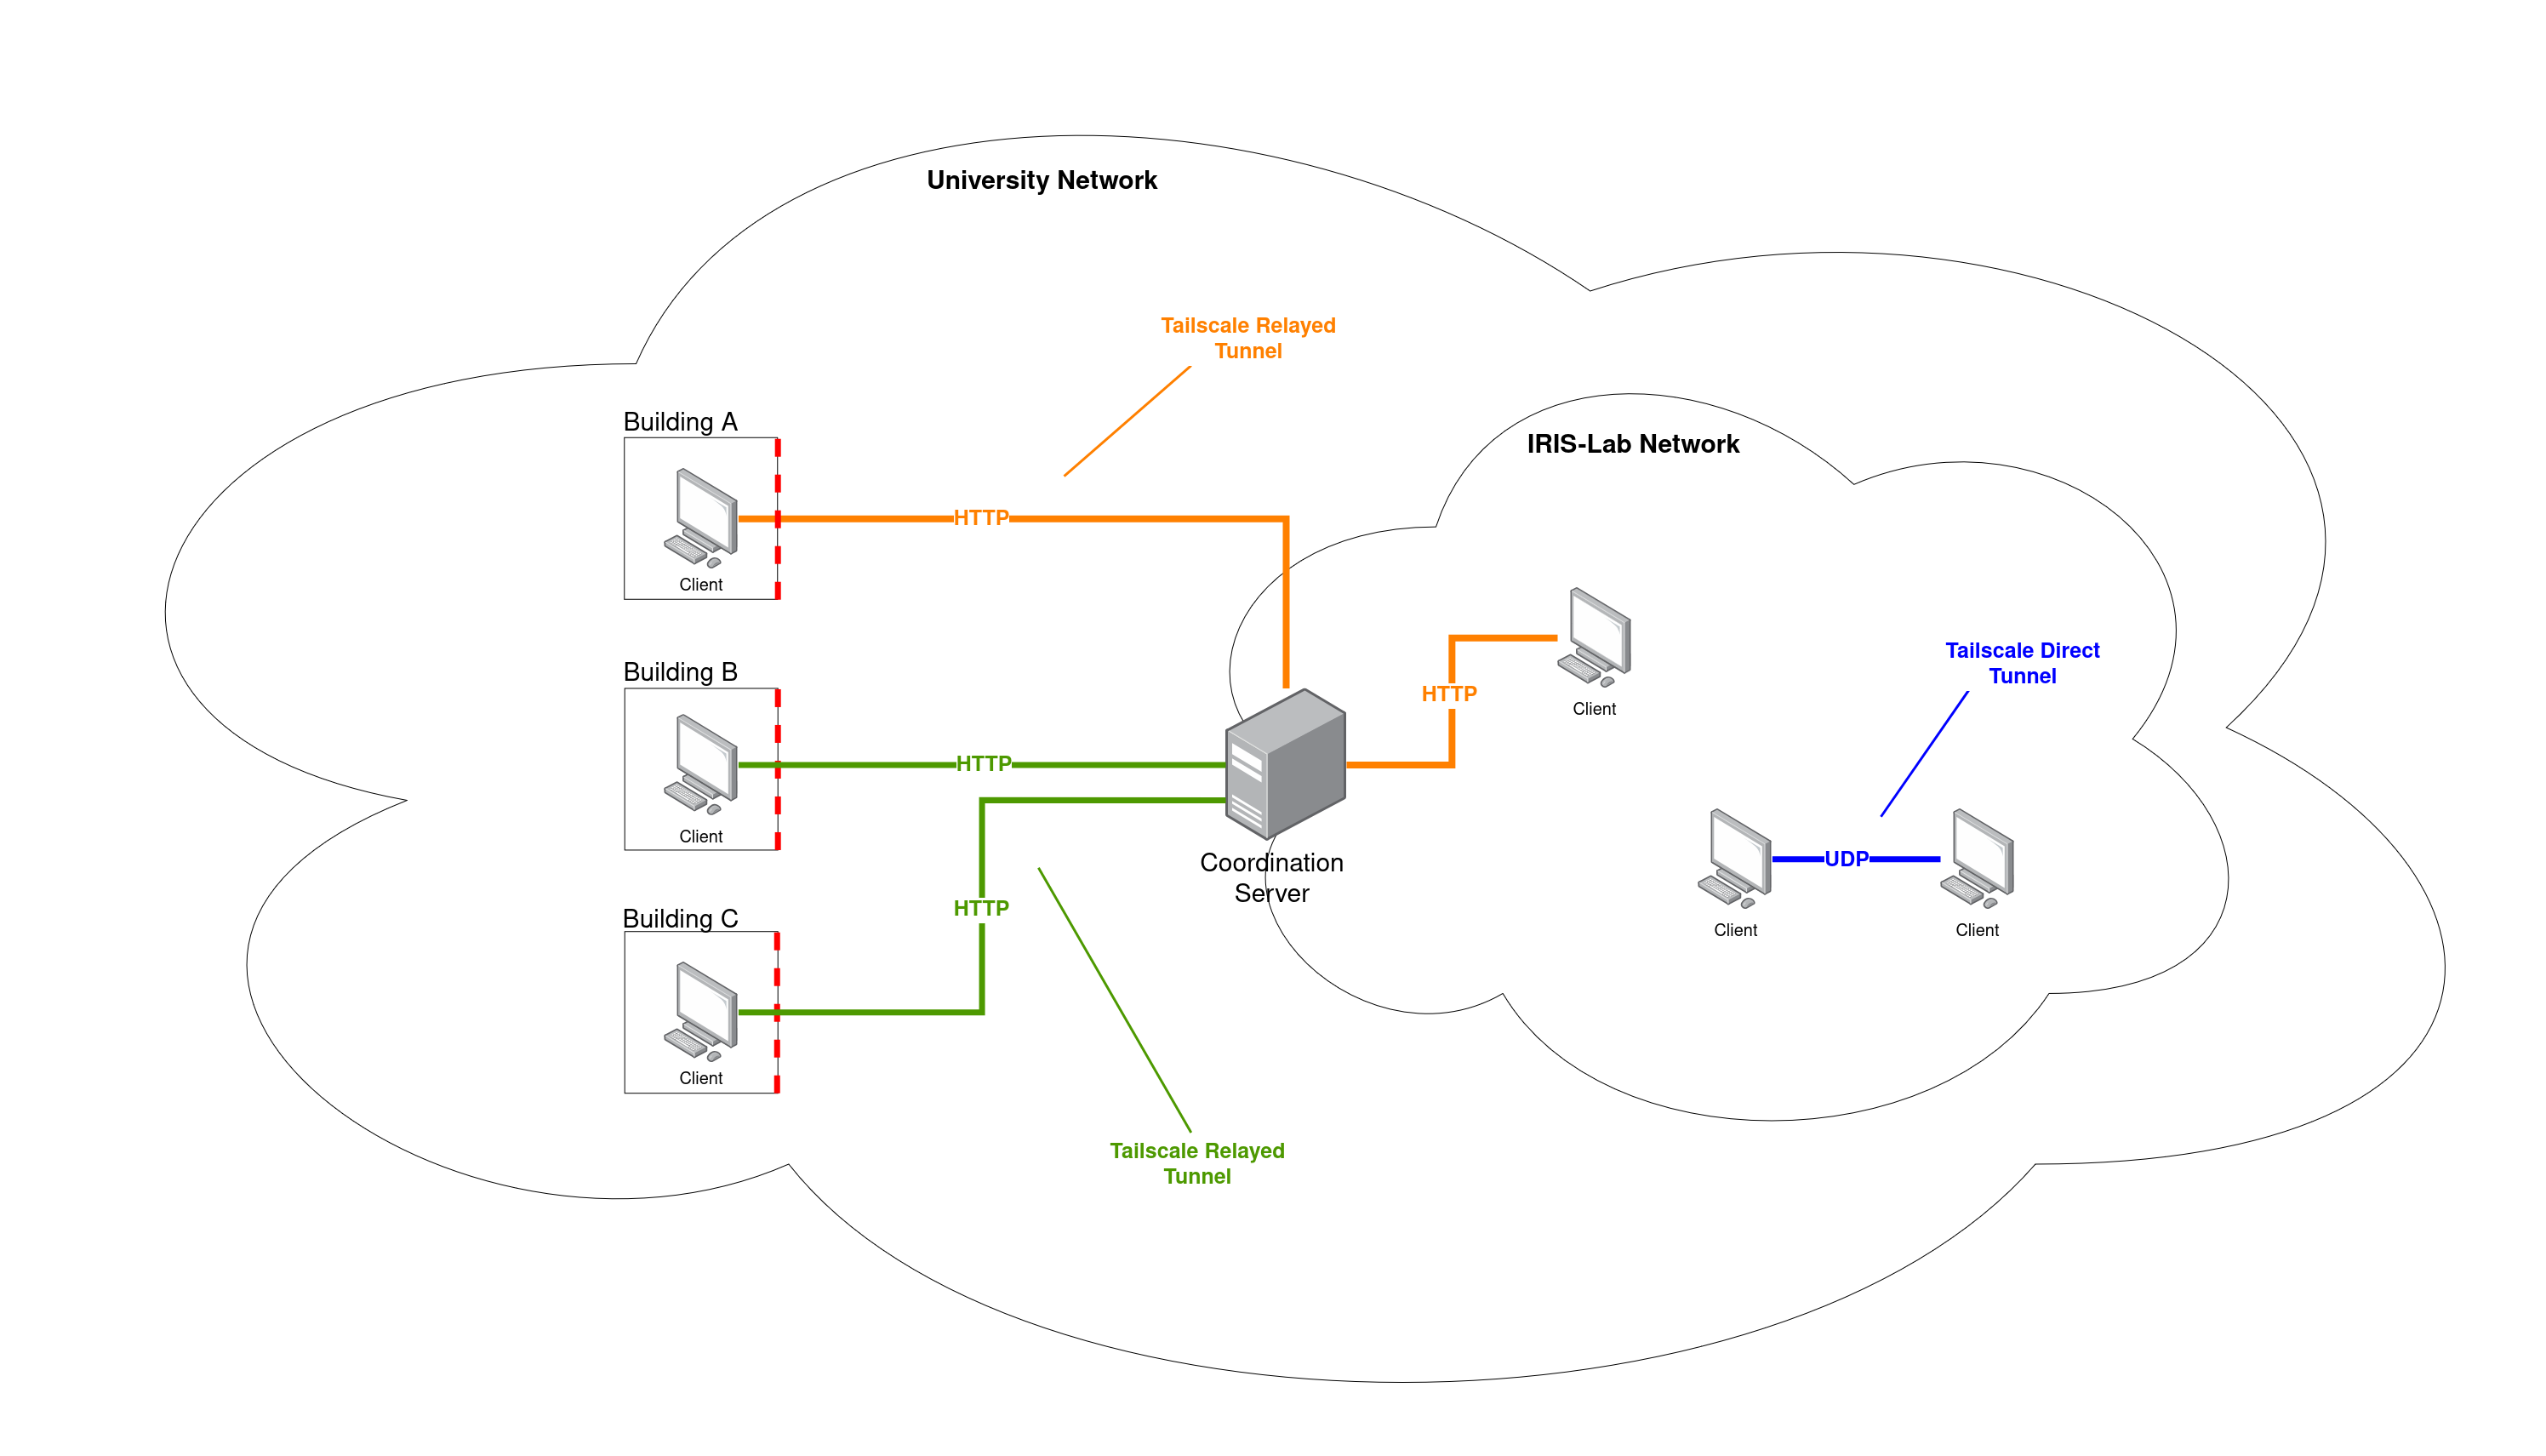
\includegraphics[width=1\textwidth]{absarch.png}
\caption{Solution's Communication Architecture. Three different scenarios can arise, identified by the blue, green and orange tunnels.}
\label{fig:absarch}
\end{figure}

To self-host a Tailscale coordination server, Headscale functions as the solution's central entity. In addition to providing a Tailscale orchestrator alternative, Headscale allows the configuration and deployment of an embedded \ac{DERP} server, which also exposes a \ac{stun} endpoint for \ac{nat}-Traversal. As such, all necessary central services are made available to clients through Headscale.

Clients run the open-source Tailscale's node software, a package containing a \ac{cli} and a daemon. Tailscale's daemon is the entity responsible for establishing and managing a client's communications both with the orchestrator and other overlay nodes, while the \ac{cli} offers an interface to control and execute operations through the daemon.

Figure \ref{fig:arch} presents the components forming both the Headscale coordination server and a Tailscale client.

\begin{figure}[h]
\centering
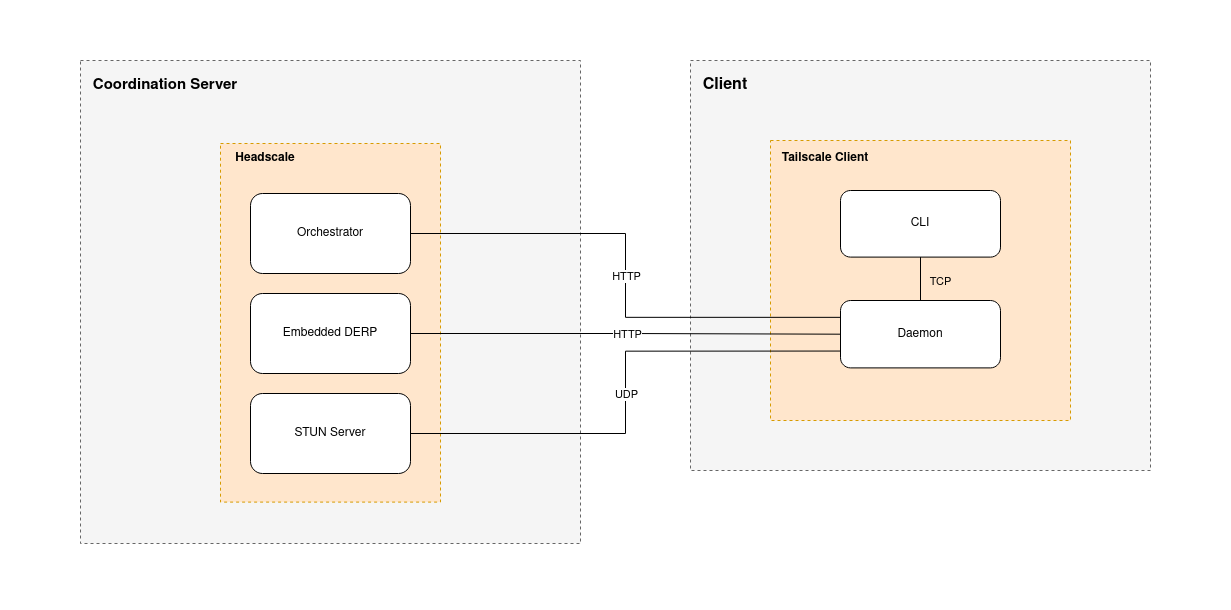
\includegraphics[width=1\textwidth]{arch.png}
\caption{Headscale coordination server and Tailscale client components}
\label{fig:arch}
\end{figure}

\subsection{Coordination Server}

The coordination server is the central entity responsible for offering clients functionalities to configure themselves, peer discovering and aid in establishing communications when dealing with highly restrictive networks. It is composed of three main services, an orchestrator, a packet relaying service and an endpoint to perform \ac{nat}-Traversal. This section explores the operations of each of these components and their respective roles in the protocol.

\subsubsection{Orchestrator}

The orchestrator provides clients with network information and services which aid in the management and establishment of secure communications. In addition to performing client authentication, authorization and key distribution, the orchestrator also ensures peer discovery, as it advertises nodes' public addresses to overlay clients. Moreover, the orchestrator facultates information regarding both \ac{stun} and \ac{DERP} listening addresses, crucial for clients to perform \ac{nat}-Traversal and establish relayed connections, respectively.

\subsubsection{Relay Server}

In Section \ref{ssec:tsnetworks}, two types of Tailscale connections were presented, direct and relayed. While the Tailscale protocol always attempts to establish direct connections first, on highly constrained networks, where \ac{nat}-traversal is unsuccessful or \ac{udp} traffic is entirely blocked by firewalls, Tailscale encapsulates encrypted packets as \ac{tcp} and transmits them to a relay server, refered to as \ac{DERP} servers, over \ac{http}. In other words, an overlay node communicating through one of such networks is able to perform this encapsulation process and forward packets to a relay. The relay server is then responsible for delivering the message to its destination. Hence, for relayed communications to be established, the orchestrator must advertise which \ac{DERP} servers are available for clients to transmit packets to.

While Tailscale's official coordination server offers a fleet of geographically distributed \ac{DERP} servers, the relay server in this solution is also a self-hosted, since our scope is to exclusevly serve \ac{ua}'s clients. Fortunately, Headscale supports the deployment of an embedded \ac{DERP} server, which runs alongside the orchestrator's main service.

\subsubsection{NAT-Traversal Server}

Finally, the coordination server is also required to expose an endpoint for clients to discover which public \ac{ip} they should advertise to the orchestrator and to perform \ac{nat}-Traversal, a  process explored in Section \ref{ss:nat-t}. Tailscale clients perform \ac{nat}-Traversal using the \ac{stun} protocol.

Clients will periodically perform \ac{ip} binding requests to a \ac{stun} server through \ac{udp} messages, receiving its respective public \ac{ip} address and port as a response. This response is then advertised and stored in the orchestrator, allowing overlay nodes to retrieve the address information of any other peer present in the network. As establishing direct communication requires knowledge of peers' public addresses, supporting \ac{nat}-Traversal is a mandatory requirement for these types of connections.

\subsection{Client}

The Tailscale client runs a daemon and a \ac{cli} to control it. Tailscale's daemon is responsible for managing a client's network connections and respective configurations, while also interacting directly with the coordination server.

\section{Implementation Details}

With the components required to self-host a complete Tailscale solution defined, this section details the implementation process. A solution was developed and deployed in two different environments, serving distinct goals. First, to obtain a better grasp of the requirements associated with self-hosting a complete Tailscale solution and to ensure compatability when using the protocol with \ac{ros} applications, a virtual environment, configured in a single host, was used. Then, for validation and performance experiments, a solution was deployed within \ac{ua}'s premises, available to any client connected to the university's network.

\subsection{Virtual Development Environment}

The virtual development environment was designed to create an analogous scenario to the one being tackled, where two clients can't immediately establish \ac{p2p} connections with each other but can both reach a public server. Hence, this environment hosts a narrow scope prototype of a self-hosted Tailscale solution. This prototype requires the deployment of an Headscale coordination server, followed by the configuration, and respective authentication, of two sample clients, using Tailscale's \ac{cli}. With the clients configured with Tailscale addresses, these can be used to run communication tests on \ac{ros} applications, through the encrypted tunnel.

\subsubsection{Environment Specification}

Such an environment was established using Oracle Virtual Box \footnote{Oracle Virtual Box, \url{https://www.virtualbox.org/}}, a general purpose virtualizer. The environment is configured with three Linux virtual machines running on minimum resources. To achieve a networking scenario analogous to the one faced by \ac{ua}'s clients, the client virtual machines are attached to individual private \ac{nat} Networks and connected via Wi-Fi to an \ac{ap}, while the coordination server virtual machine is attached to a network bridge on the host's Ethernet interface. Figure \ref{fig:sandbox} depicts this topology. This networking configuration creates a situation where both clients have no knowledge of each other nor endpoints to communicate through, but are able to directly reach the coordination server. Obviously, this simulation of the networking conditions can't be entirely accurate, since, as referenced in section \ref{sec:uanet}, details regarding \ac{ua}'s network mechanisms are vastly unknown. It is possible, however, to create a similar situation, where clients can't immediately form \ac{p2p} communications with each other but can all communicate with an external, public server. Moreover, as stated in previous sections, Tailscale's protocol efficiently deals with most network constraints preventing direct communication. In other words, it is only known clients can't communicate, the reasons behind why they can't are abstracted by Tailscale.

\begin{figure}[h]
\centering
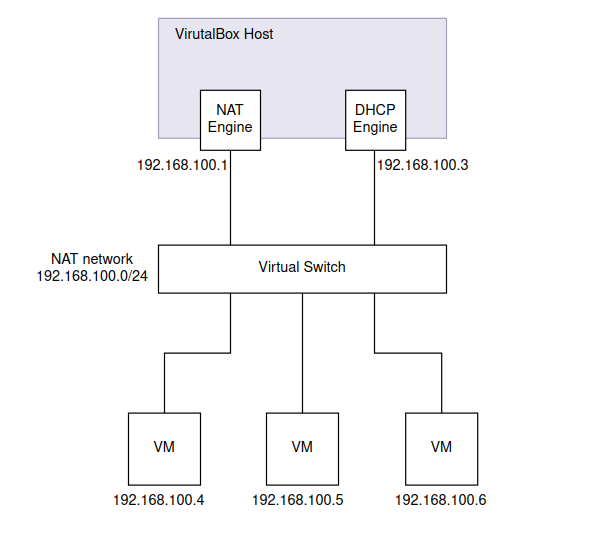
\includegraphics[width=0.5\textwidth]{dev.png}
\caption{Virtual Development Environment Architecture}
\label{fig:sandbox}
\end{figure}

The access point used in this environment is a N600 Wireless Dual Band Gigabit router. The host machine is connected to the access point via Ethernet. With this setup, when one of the client machines wants to communicate with \textbf{VM-3}, traffic will be routed from the client to the \ac{ap}'s Wi-Fi interface. Then, the router will forward the packet through its Ethernet interface, reaching the host machine and, consequently, reaching \textbf{VM-3}, as its network adapter is bridged to the host's Ethernet interface.

The three virtual machines composing the environment run \emph{Ubuntu Server 22.04} as their operating system. Due to the nature of the goals to be achieved in this phase, which focus on an extremely narrow scope, the machines require very little resources. Regarding networking, \textbf{VM-3} is attached to a bridge network on the Ethernet interface of the host machine. As for \textbf{VM-1} and \textbf{VM-2}, each respective network adapter is attached to a \ac{nat}, isolating clients on their own private networks, inaccessible from the outside. All machines can access the internet through the access point. Both \textbf{VM-1} and \textbf{VM-2} are assigned the same private \ac{ip} address since they are residing in distinct private networks.

Table \ref{table:vmspecs} summarizes the virtual machines' configuration.

\begin{table}[]
\centering
\resizebox{\textwidth}{!}{
     \begin{tabular}{c|c|c|c|c|}
     \cline{2-4}
     \multicolumn{1}{l|}{}                           & \textbf{VM-1}        & \textbf{VM-2}        & \textbf{VM-3}        \\ \hline
     \multicolumn{1}{|c|}{\textbf{Operating System}} & Ubuntu Server 22.04 & Ubuntu Server 22.04 & Ubuntu Server 22.04 \\ \hline
     \multicolumn{1}{|c|}{\textbf{Memory (Mb)}}      & 1024                & 1024                & 1024                \\ \hline
     \multicolumn{1}{|c|}{\textbf{Storage (Gb)}}     & 10                  & 10                  & 10                  \\ \hline
     \multicolumn{1}{|c|}{\textbf{CPUs}}             & 1                   & 1                   & 1                   \\ \hline
     \multicolumn{1}{|c|}{\textbf{Network Adapter}}  & NAT                 & NAT                 & Bridged (ethernet)  \\ \hline
     \multicolumn{1}{|c|}{\textbf{Address}}          & 10.0.2.15           & 10.0.2.15           & 192.168.10.214      \\ \hline
     \end{tabular}
}
\caption{Development Virtual Machines specification}
\label{table:vmspecs}
\end{table}

\subsubsection{Headscale Instance Deployment}
\label{sec:devhs}

Headscale provides a configurable open-source implementation of Tailscale's coordination server. At the time of writing, the latest stable Headscale release is \emph{v0.22.3} \footnote{Headscale's official releases, hosted in GitHub. https://github.com/juanfont/headscale/releases.}, which is the version of the software referred to in the rest of this document.

The Headscale instance must be made available to all clients. In this environment, that means Headscale is deployed in \textbf{VM-3}, since the two other Virtual Machines can communicate with it directly. Hence, in this public server, an Headscale instance was deployed, following the official documentation's guidelines \footnote{Headscale's online documentation. https://headscale.net/running-headscale-linux/ }

Headscale includes in its software package a YAML file used to configure coordination server's parameters. First, the \textbf{server\_url} field, which dictates the endpoint clients should connect to for authentication, points to \textbf{VM-3}'s \ac{ip} address, 192.168.10.214, on port 8080, where Headscale's main orchestrator service is listening. Regarding Tailscale \ac{ip} assignments, this instance uses the default subnet prefixes, 100.64.0.0/10 for ipv4 and fd7a:115c:a1e0::/48 for ipv6. Registered clients will be assigned \ac{ip} addresses in these ranges. For the scope of this environment, no other additional configurations are necessary.

With the service running, \textbf{VM-3} is now listening for Tailscale clients to connect and start using the protocol. To perform authentication, clients are required to login under a user. By default, Headscale does not create any users automatically. For development purposes, an Headscale user, \textbf{dev}, was created in the instance and shall be the user clients will register themselves under.

\subsubsection{Client Deployment}

Initially, clients can't really establish a direct connection in a traditional way. In fact, neither client is assigned a public address which could be used as a communication's endpoint, nor do they possess any information regarding one another. They can, however, reach the outside Internet, which consequently implies the translation of their private addresses into public ones, a process carried by the adapter attached to the host machine's \ac{nat}. In section \ref{ssec:tsnetworks}, Tailscale's support for \ac{nat}-Traversal was explored. Thus, a Tailscale client is able to obtain its public \ac{ip} and port by querying a \ac{stun} server and announce it to the control server. With both clients' public addresses stored, when communication is attempted, Tailscale will keep \ac{nat} holes open, allowing for a bidirectional flow of packets to be possible, through the public \acp{ip} addresses.

Hence, the Tailscale binaries were installed in each client, using Tailscale's install shell script \footnote{Tailscale's install script, publicly available online. https://tailscale.com/install.sh}.

At this point, clients are ready to perform authentication in the coordination server using the Tailscale's \ac{cli} and start communicating through Tailscale tunnels.

\subsubsection{Authentication}

Authenticating in the Headscale instance can be done either using a pre-authenticated key, generated by the coordination sever and shared with a client, or by accessing the instance through the browser in the client side. For automation purposes, the authentication keys provide a much more useful mechanism.

With that said, reusable keys were generated in the control server with Headscale's \textbf{headscale preauthkeys create}, an utility included in the software's \ac{cli}, and shared with its respective clients. The client machines are now able to authenticate by using the \textbf{tailscale up} command. Two additional command-line parameters are set, the \emph{login-server}, which points to the address previously defined in Headscale's config's \textbf{server\_url}, and the \emph{authkey}, where the shared pre-authenticated key is injected.

With the clients authenticated, both devices are respectively assigned a Tailscale IP and hostname. Table \ref{tab:tsips} presents both clients' Tailscale configurations. At this state, a direct connection can be established via Tailscale interfaces.

\begin{table}[]
\centering
\begin{tabular}{c|c|c|}
\cline{2-3}
\textbf{}                                         & \textbf{VM-1} & \textbf{VM-2} \\ \hline
\multicolumn{1}{|c|}{\textbf{Tailscale Hostname}} & dev-1         & dev-2         \\ \hline
\multicolumn{1}{|c|}{\textbf{Tailscale IP (v4)}}  & 100.64.0.1    & 100.64.0.2    \\ \hline
\multicolumn{1}{|c|}{\textbf{Tailscale IP (v6)}}  & fd7a:115c:a1e0::1     & fd7a:115c:a1e0::2         \\ \hline
\end{tabular}
\caption{Clients' Tailscale configuration after authentication}
\label{tab:tsips}
\end{table}

\subsubsection{Communication with ROS}

With both clients up and communicating, our last validation in this environment aims to ensure the connections are compatible with the \ac{ros} middleware. Therefore, a very simple \ac{ros} scenario was deployed in the clients. As the scope for this experiment lies solely on validating communication through Tailscale in a \ac{ros} context, clients are only required to run a very basic \ac{ros} distribution, hence, a no-GUI package, \textbf{ros-noetic-ros-base} \footnote{ROS-Base (Bare Bones). Basic ROS packaging, build and communication libraries. No GUI. Pulled from public repositories.} was installed in both clients.

The experiment starts by configuring \textbf{VM-1} as a \ac{ros} Master, with the \textbf{ros-core} command which automatically assigns the client as the new master, listening on port 11311, under the \textbf{ROS\_HOSTNAME} dev-1, matching its Tailscale hostname for convenience. Then, \textbf{VM-2} must acknowledge \textbf{VM-1} as the \ac{ros} master. The \textbf{ROS\_MASTER\_URI} environment variable points to where the \ac{ros} Master is listening. So, \textbf{VM-2} sets this variable with \textbf{VM-1}'s \ac{ros} \ac{uri}, which is composed by \textbf{VM-1}'s hostname, dev-1, and the previously established \ac{ros} port, 11311.

\textbf{VM-2} successfully configures its \ac{ros} ecosystem acknowledging \textbf{VM-1} as its master, effectively validating the use of Tailscale tunnels in conjunction with the \ac{ros} middleware.

\subsection{Pilot Environment}

The following section presents the configuration and deployment of a solution capable of being used by any client in the campus. As such, and as mentioned before, this implies that the Headscale instance must be available regardless of a client's physical location within \ac{ua}'s premises.

\subsubsection{Headscale Deployment}
\label{ssec:hs}

In this solution, the Headscale instance is hosted within \ac{iris}'s network. Table \ref{tab:hsresources} presents the server machine's resources. This, however, only allows communications from clients residing in the laboratory's private network. For clients to be able to reach the instance from any location in the campus, port forwarding rules were created on an exposed server in \ac{iris}'s network, available to any client connected to \ac{ua}'s network. This server forwards traffic on ports \ac{tcp}/8080, for the main Headscale service and the embedded \ac{DERP} and \ac{udp}/3478, for the \ac{stun} protocol, to the Headscale server. With this configuration, clients within the campus, which can directly reach the public facing relay machine via \ac{http}, can perform authentication in the Headscale instance. Figure \ref{fig:prodsolution} depicts such architecture.

\begin{table}[]
\centering
\begin{tabular}{c|c|}
\cline{2-2}
\multicolumn{1}{l|}{}                           & \textbf{Coordination Server}                                  \\ \hline
\multicolumn{1}{|c|}{\textbf{Operating System}} & \begin{tabular}[c]{@{}c@{}}Ubuntu Server\\ 22.04\end{tabular} \\ \hline
\multicolumn{1}{|c|}{\textbf{Memory (Gb)}}      & 16                                                            \\ \hline
\multicolumn{1}{|c|}{\textbf{Storage (Gb)}}     & 60                                                            \\ \hline
\multicolumn{1}{|c|}{\textbf{CPUs}}             & 4                                                             \\ \hline
\multicolumn{1}{|c|}{\textbf{Address}}          & 192.168.1.7                                                   \\ \hline
\end{tabular}
	\caption{Pilot environment's coordination server resources}
	\label{tab:hsresources}
\end{table}

\begin{figure}[h]
\centering
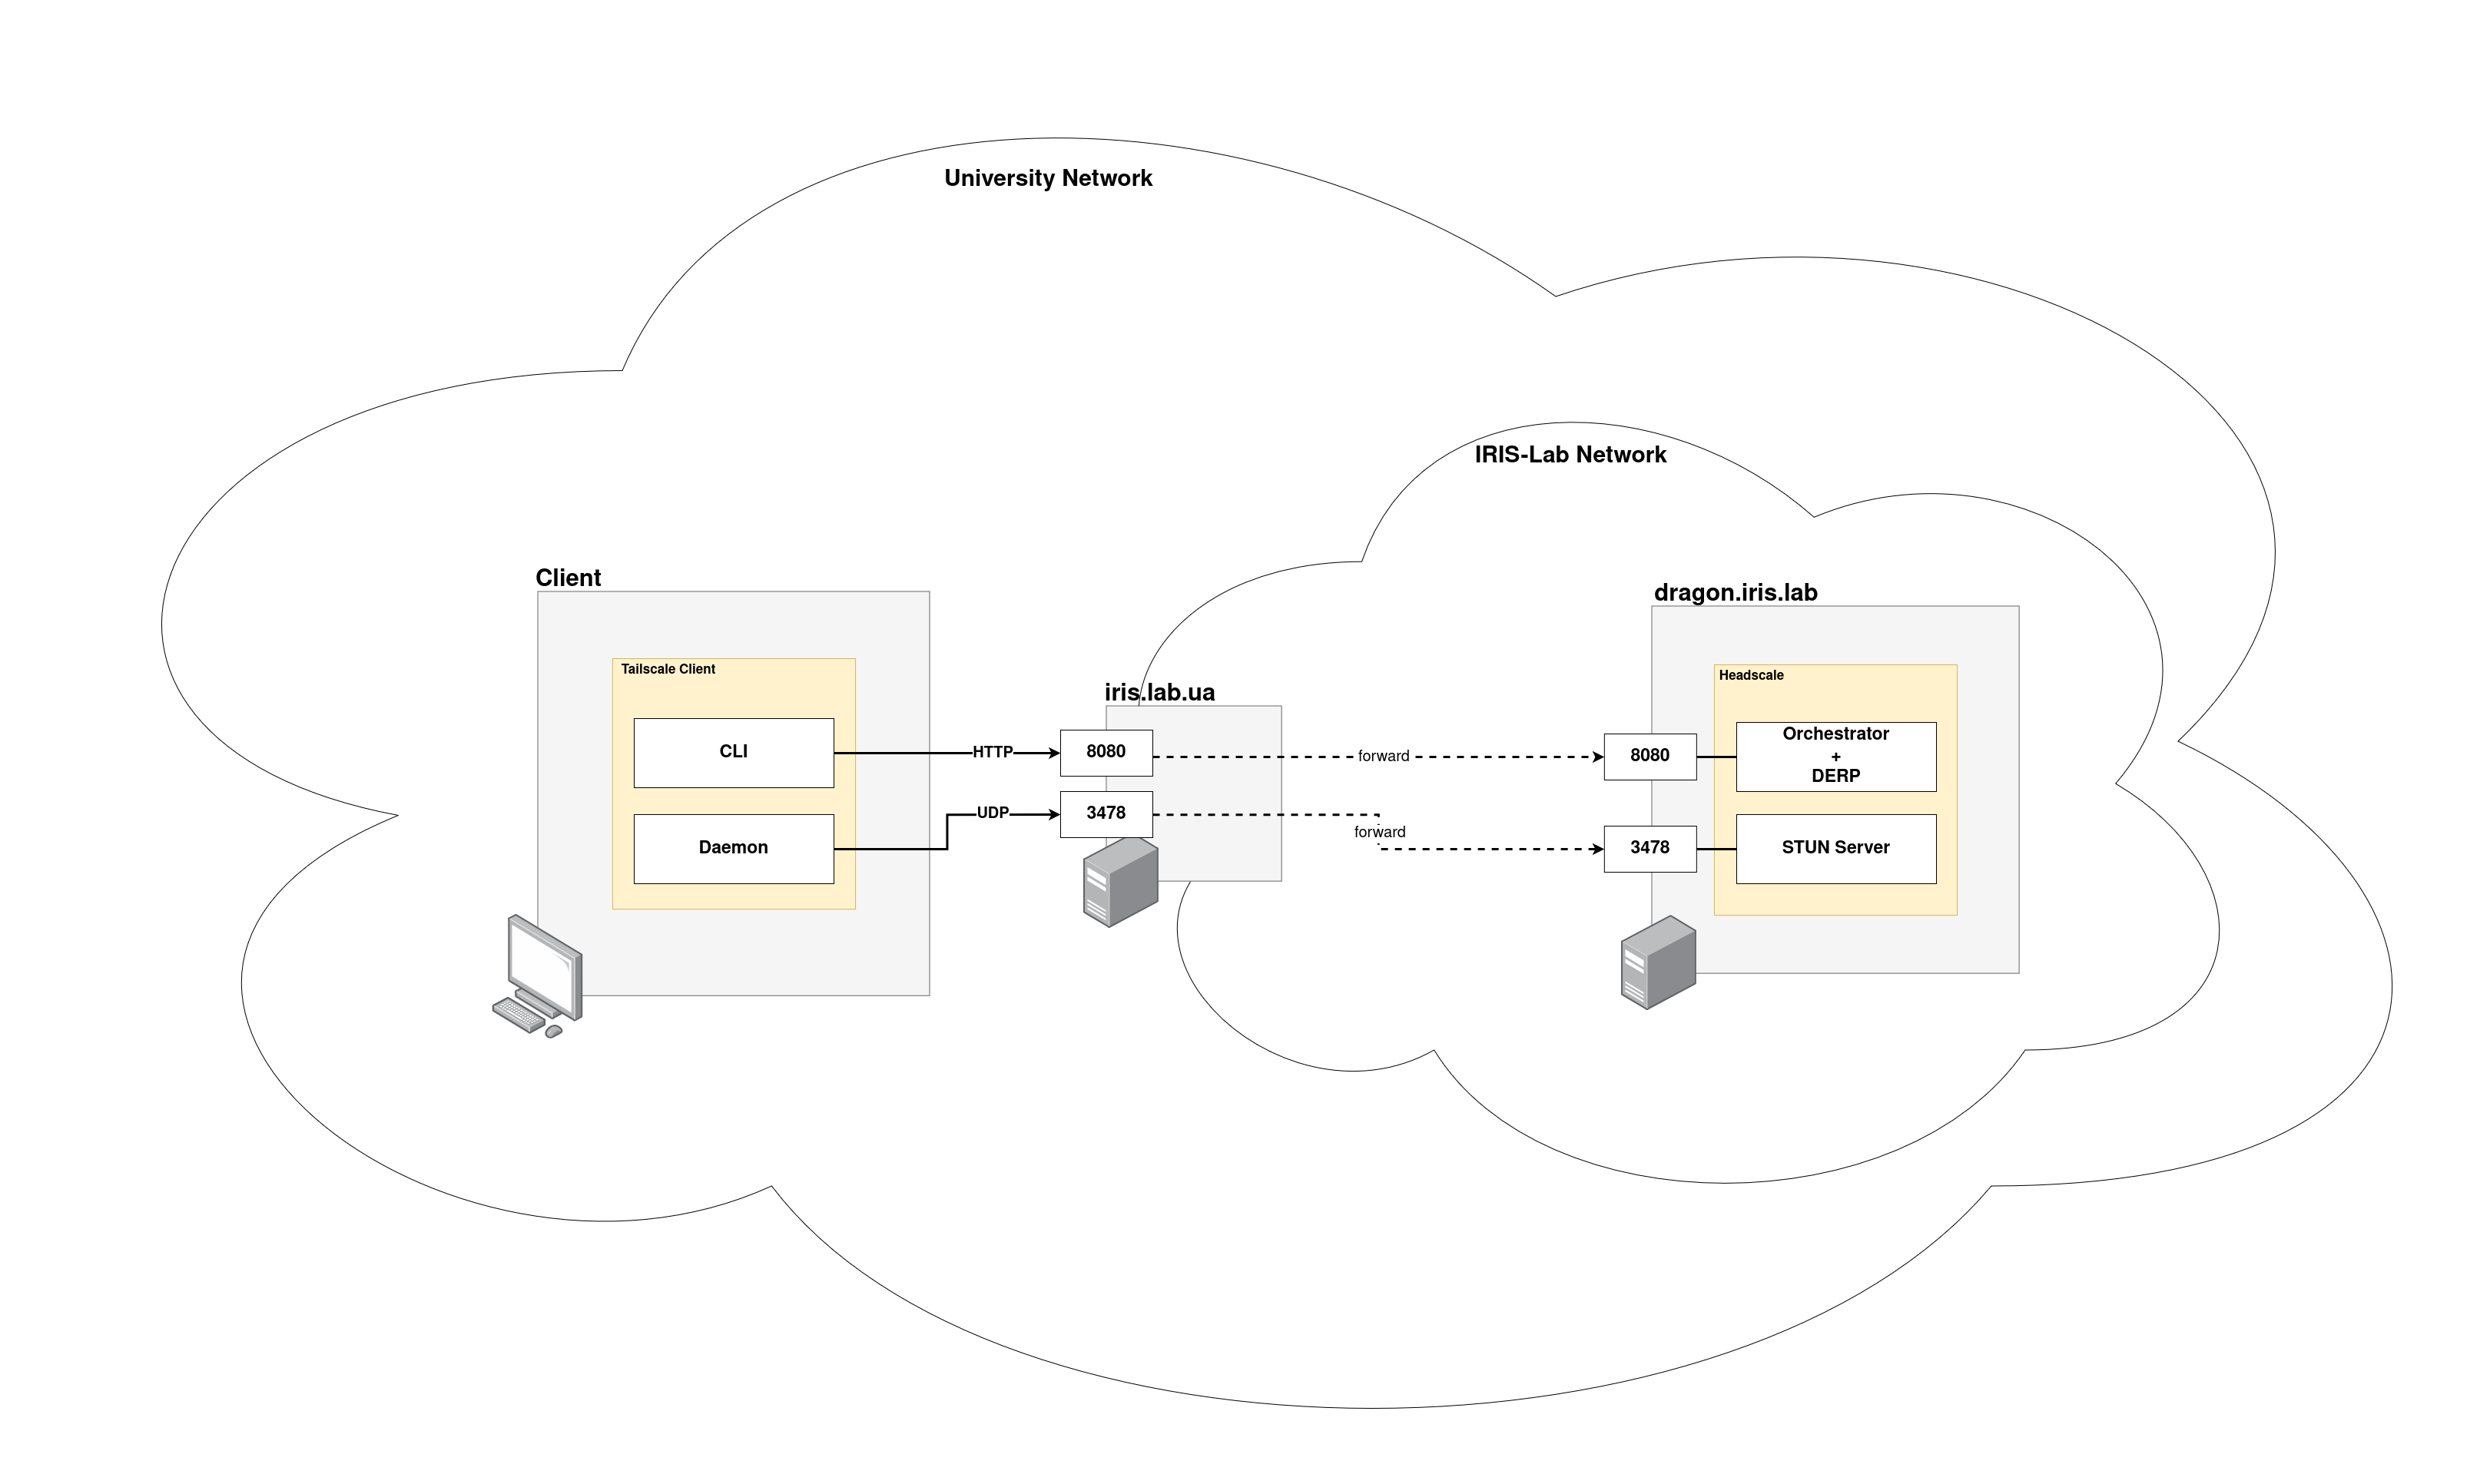
\includegraphics[width=\textwidth]{pilot.png}
\caption{Pilot Environment Deployment Diagram}
\label{fig:prodsolution}
\end{figure}

Since the coordination server's host also runs Ubuntu in this environment, deployment followed the process described in the development environment (see Section \ref{sec:devhs}). Regarding configuration, however, the \textbf{server\_url} parameter, which points to the endpoint clients should use to authenticate, is now set as the \ac{fqdn} of the proxy server, \emph{iris-lab.ua.pt}.

Initially, Headscale was configured to use Tailscale's \ac{DERP} server fleet. However, upon testing this scenario, relayed connections implied the redirection of traffic to a \ac{DERP} server in Germany, resulting in tunnels with an average \ac{rtt} of 452ms, a value unacceptable for the scope of this dissertation. Moreover, as this solution is meant to be used exclusively by \ac{ua}'s clients, traffic should be contained within the campus' network. Therefore, Tailscale's \ac{DERP} fleet was discarded, opting for a self-hosted alternative.

Headscale allows the use of an embedded \ac{DERP} server, which also exposes \ac{stun} functionalities for \ac{nat}-Traversal. This server can be enabled through Headscale's configuration file, and runs alongside Headscale's main orchestrator service, on the same address and port. As for the \ac{stun} endpoints, these are also configured to run in the same address, on \ac{udp} port 3478.

Using the embedded self-hosted \ac{DERP} allows relayed communication between clients to be much more efficient, with more appealing latencies, discussed further in Chapter \ref{chap:results}.

To use the self-hosted \ac{DERP} server, Headscale is required to be exposed on an \ac{https} server, hence it needs a valid X509 certificate. Although Headscale's configuration allows a seamless integration with certification tools such as \ac{le} or Caddy, in this scenario, where Headscale's \ac{fqdn} is not public, such methods aren't as straightforward. Alas, to certify Headscale, self-signed certificates were generated using the \textbf{openssl} \ac{cli} and added manually to the instance, by pointing to both certificate and key file paths through Headscale's configuration file.

Using self-signed certificates requires additional client certificate trust configurations, covered in the following sections.

\subsubsection{Client Deployment}

Regarding client configurations, Headscale's certificate needs only to be added to the client machine's trusted list. On Debian distributions, this required moving the certificate to the \emph{/usr/local/share/ca-certificates} directory and updating the list with the command \textbf{update-ca-certificates}. With the coordination's server certificate added to the trust chain, a peer is able to use the protocol by running the official Tailscale client software.

\subsection{Automation}

This chapter details the development of automation tools to speed up deployment and configuration processes. Two main goals were achieved, related to automatic deployments of the control server and clients. First, automating the deployment of a configured Headscale instance. This implies automating software installation, configuration applying and certificate management. Regarding clients, deployments require Tailscale client installation, adding Headscale's certificate to the trust list and, finally, authenticate in the control server.

All scripts discussed in the following paragraphs are available on a GitHub repository. \footnote{UA Overlays Automation repository: https://github.com/VascoRegal/ua-overlays-automation}

\subsubsection{Headscale Deployment}

Headscale's deployment requires both the installation of the software and its configuration, namely the configuration YAML and the server certificate.

Hence, the \textbf{install\_headscale.sh} shell script starts by downloading a desired Headscale package, where version and system architecture are specified with command-line arguments. Then, the script fetches the Headscale's configuration YAML, publicly available in the automation repository, and applies it to the instance. Finally, the certificate is generated with the \textbf{openssl} \ac{cli} and placed, along with the certificate's key, in its respective path (matching what was defined in the the YAML).

\subsubsection{Client Deployment}

A shell script was also created for the clients. Here, configuring a client requires the installation of the Tailscale client package, running the already covered official install script. Finally, Headscale's server certificate is fetched and added to the system's trust mechanisms.

Running this simple script leaves a machine in a state where, given a pre-shared key, authentication can be performed with the \textbf{tailscale up} command.

\chapter{Experiments and Results}
\label{chap:results}

In order to validate the developed solution, several experiments were conducted which provide insights regarding the overlay networks' communication performance, security and usability in the context of \ac{ros} applications. Hence, this chapter details the procedures taken for results and metrics gathering, followed by their respective analysis and derived conclusions.

\section{Network Performance}

Network performance is understood as the quality of the communication in the eyes of an overlay node. Measuring network performance requires the collection  and visualization of metrics produced while data is being exchanged on the overlay networks. For the scope of our conclusions, four of such metrics were gathered, on connections happening in distinct scenarios.

The metrics we chose for this experiment provide insights on three distinct dimensions, outlined in ~\cite{livronet, Hanemann2006}.

\subsubsection{Delay}

Delay in network performance is a dimension refering to the time packets take to be transmitted from a source to a destination, through its communication medium. Network congestion, insufficient computational resources and routing rules directly influence network delay. To measure the delay associated with a connection, two metrics are considered, Round Trip Time (\ac{rtt}) and jitter.

\ac{rtt} times dictate how long a source has to wait to receive a response from its destination, while jitter measures the variation of packet arrival times. High jitter has an impact on the smoothness of a connection, generally having noticeable negative effects on real time communications and media streaming \cite{claypool1999effects}.

\subsubsection{Bandwidth and Throughput}

Bandwidth is a dimension perceived as the maximum amount of information capable of being transmitted through a connection in a given time interval. Throughput, while also measuring the amount of transmitted data over time, represents how much data in a given communication is actually transferred by unit of time. In other words, measuring throughput allows us to understand the rate at which data is transmitted between a source and a destination, while bandwidth measures the network's total capacity. Network throughput can be calculated by executing several packet transmissions between any two nodes and measuring how much information is successfully transmitted over a given time delta.

\subsubsection{Losses and Errors}

Finally, this dimension tackles how much information is not correctly transmitted and is measured by calculating a communication's packet loss, the fraction of packets sent which don't arrive at a destination. Losing packets implies data retransmission, which contributes negatively to the overall network performance.

\subsection{Metric Gathering}
\label{ss:metrics}

The metrics to be gathered for network performance analysis are \textbf{\ac{rtt}} and \textbf{jitter} regarding delays, \ac{tcp} \textbf{throughput} for information transfer rate and \textbf{packet loss} to assess any issues regarding packets not being properly transmitted.

There are numerous open source tools which measure most of these metrics by running configurable network tests. One such example is iperf \footnote{iPerf - The TCP, UDP and SCTP network bandwidth measurement tool, \url{https://iperf.fr/}}. Iperf operates by exchanging packets through a client-server model and offers tests capable of collecting both \ac{tcp} and \ac{udp} throughput and bandwidth, network jitter and packet loss. \ac{rtt} times can be calculated by exchanging a given number of \ac{icmp} packets and measuring communication travel times, achievable with simple \textbf{ping} commands.

These processes were automated using a python script \footnote{https://github.com/VascoRegal/ua-overlays-automation/blob/main/tests/network/iperf/run.py}. This script starts by connecting to an iperf server and running \ac{tcp} and \ac{udp} iperf tests, outputting its results as \ac{json}. Then, to the same host running the iperf server, \ac{icmp} packets are exchanged, calculating \ac{rtt} minimum, maximum, mean and deviation values, which are also appended to the previously produced \ac{json} object. These results are finally exported to a file for later processing. The duration of each iperf test and the total number of \ac{icmp} packets exchanged for \ac{rtt} calculations are both configurable variables.

The result files produced by running this script allows us to build a dataset containing necessary metrics, used to draw the conclusions present further in this chapter.

\subsection{Network Performance Experiments}
\label{ss:netperf}

Having defined the relevant metrics to evaluate communication performance through the overlays and development of a script which automates the results gathering processes, experiments are ready to be run between any two overlay nodes. Since communication is possible through Tailscale relayed connections regardless of clients' physical locations, we can collect insights from multiple campus points. This will not only allow us to understand the performance of the solution and how it behaves with geographical distance but also ensure the overlays can be used from anywhere within \ac{ua}'s premises.

For these experiments, an overlay node running an iperf server was deployed in \ac{iris}, connected to \ac{ua}'s network. Then, with another machine, the experiment script was run, pointing the iperf server as the \ac{iris}'s node's Tailscale \ac{ip}, from disperse campus' locations. Table \ref{tab:locs} presents the selected test case buildings.

Regarding test configuration, both \ac{tcp} and \ac{udp} iperf tests were run for 10 minutes each. Regarding \ac{rtt} calculations, a total of 100 \ac{icmp} replies were used.


\begin{table}[]
  \centering
\begin{tabular}{|c|c|c|}
\hline
\textbf{Location}                                                                                             & \textbf{\begin{tabular}[c]{@{}c@{}}Building\\ ID\end{tabular}} & \textbf{\begin{tabular}[c]{@{}c@{}}Connection\\ Type\end{tabular}}     \\ \hline
\begin{tabular}[c]{@{}c@{}}University Library\\ (BIB)\end{tabular}                                          & 17                                                                 & \begin{tabular}[c]{@{}c@{}}Tailscale\\ (relayed)\end{tabular} \\ \hline
\begin{tabular}[c]{@{}c@{}}Eletronics, Telecomunications and Informatics\\ Department\\ (DETI)\end{tabular} & 4                                                                  & \begin{tabular}[c]{@{}c@{}}Tailscale\\ (relayed)\end{tabular} \\ \hline
\begin{tabular}[c]{@{}c@{}}Pedagogical Complex\\ (CP)\end{tabular}                                            & 23                                                                 & \begin{tabular}[c]{@{}c@{}}Tailscale\\ (relayed)\end{tabular} \\ \hline
\begin{tabular}[c]{@{}c@{}}Mathematics Department\\ (DMAT)\end{tabular}                                     & 11                                                                 & \begin{tabular}[c]{@{}c@{}}Tailscale\\ (relayed)\end{tabular} \\ \hline
\begin{tabular}[c]{@{}c@{}}Biology Department\\ (DBIO)\end{tabular}                                         & 8                                                                  & \begin{tabular}[c]{@{}c@{}}Tailscale\\ (relayed)\end{tabular} \\ \hline
\begin{tabular}[c]{@{}c@{}}Economics and Management Department\\ (DEGEIT)\end{tabular}                      & 10                                                                 & \begin{tabular}[c]{@{}c@{}}Tailscale\\ (relayed)\end{tabular} \\ \hline
\begin{tabular}[c]{@{}c@{}}Exhibition Hall\\ (EXPO)\end{tabular}                                              & 24                                                                 & \begin{tabular}[c]{@{}c@{}}Tailscale\\ (relayed)\end{tabular} \\ \hline
\end{tabular}
\caption{Locations used for network performance analysis}
\label{tab:locs}
\end{table}

\subsection{Results}

The metrics collected from each building are presented in Table \ref{tab:perfres}.

\begin{table}[h!]
\centering
\begin{tabular}{|c|c|c|c|c|c|}
\hline
\multirow{Building} & \multicolumn{3}{c|}{\begin{tabular}[c]{@{}c@{}}Round-Trip Time \\ (ms)\end{tabular}} & \multirow{\begin{tabular}[c]{@{}c@{}}Average TCP Throughput \\ (Mbit/s)\end{tabular}} & \multirow{\begin{tabular}[c]{@{}c@{}c@{}}Average \\ Network Jitter\\ (ms)\end{tabular}} \\ \cline{2-4}
                            & Min & Mean & Max &                       &                         \\ \hline
DMAT & 8.24 & 22.37 & 240.9 & 45.874 & 0.859  \\ \hline
DEGEIT & 7.85 & 19.23 & 244.05 & 49.615 & 1.119  \\ \hline
CP & 7.63 & 19.43 & 239.96 & 43.061 & 0.834  \\ \hline
BIB & 7.94 & 12.88 & 45.17 & 46.849 & 0.764  \\ \hline
DBIO & 0 & 0 & 0 & 0 & 0 \\ \hline
DETI & 8.41 & 20.01 & 265.88 & 31.744 & 11.854  \\ \hline
EXPO & 7.63 & 17.06 & 219.88 & 33.685 & 2.843  \\ \hline
\end{tabular}
\caption{Solution's network performance results from various campus' buildings.}
\label{tab:perfres}
\end{table}

\iffalse
\begin{figure}[h]
\centering
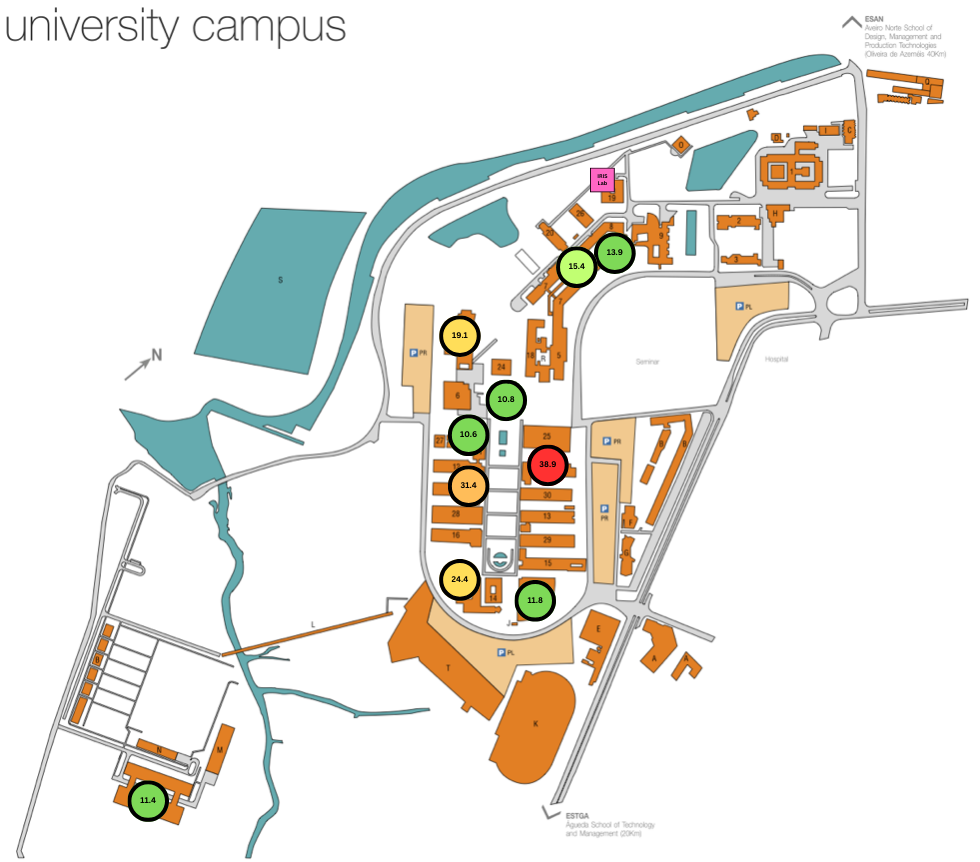
\includegraphics[width=0.8\textwidth]{ua-latency.png}
\caption{Average RTT on a Tailscale connection from different UA buildings to IRIS-Lab. The numbers in the circles represent average RTT values, in ms.}
\label{fig:ualats}
\end{figure}
\fi

\section{Protocol Overhead}

Communicating with the Tailscale protocol implies additional operations  to take place on sending and receiving data, which introduces an overhead to the general network performance. In fact, data encryption, security mechanisms and transmission of additional Tailscale protocol packets produce a toll on the regular network behaviour. Moreover, since connections within the university's network are relayed, meaning traffic is being redirected over \ac{http}, an additional degradation of network performance is also expected. To understand this dimension, this section presents an experiment which provides insights on said protocol overhead, regarding network delay and throughput.

This experiment aims to measure Tailscale's overhead on communication, by interpolating data collected, under very similar conditions, from a connection through a regular Wi-Fi interface against a connection done through Tailscale tunnel.

Such a scenario can be achieved with two clients residing inside \ac{iris}. With both machines connected to \ac{iris}'s private network, they can communicate directly via private \acp{ip}, hence metrics were collected with the script described in Section \ref{ss:metrics}. Then, the same metric gathering was run for the same scenario, with one of the clients connected to \ac{ua}'s network and the test done via Tailscale \acp{ip}.

\subsection{Results}

The two generated datasets allow us to visualize how Tailscale impacts network performance. Figure \ref{fig:overhead} presents the \ac{tcp} throughputs for the both experiments, while figure \ref{fig:latency_overhead} compares the \ac{rtt} distributions. Analysing the figures corroborates the idea that communicating through relayed Tailscale connections implies a considerable loss in network performance. To be able to represent this performance depletion numerically, we can calculate the relative change between the two measurements, using the percent log-change formula \cite{tornqvist1985should}.

The percent log-change is a numerical indicator of the change between two groups of values. In the context of this analysis, the percent log-change represents how much throughput was lost and how \ac{rtt} times increased, when comparing the internal and tunnel connections. We chose to use the log-change as an indicator instead of directly calculating the percentage change as it outputs a symmetric indicator, abstracting the necessity of choosing one connection as the baseline. The percent log-change is given by the expression:

\[
\text{Log-Change (\%)} = \ln\left(\frac{y}{x}\right) \times 100
\]

Where \textbf{y} and \textbf{x} are the two set of values under comparison. Using the average measurements generated by the network tests, throughput loss can be calculated with the expression:

\[
\text{Throughput Loss (\%)} = \ln\left(\frac{\overline{\text{TP}}_I}{\overline{\text{TP}}_T}\right) \times 100
\]

Where \textbf{ \( \overline{\text{TP}}_I \)} is the average throughput for the internal connection and \textbf{\( \overline{\text{TP}}_T \)} is the average throughput for the Tailscale connection, which results in a throughput loss of \textbf{46.23} \%

The same procedure can be applied to the measured \ac{rtt} values:

\[
\text{RTT Increase (\%)} = \ln\left(\frac{\overline{\text{RTT}}_I}{\overline{\text{RTT}}_T}\right) \times 100
\]

Similarly, \textbf{ \( \overline{\text{RTT}}_I \)} is the average \ac{rtt} times for the internal connection while \textbf{\( \overline{\text{RTT}}_T \)} is the average \ac{rtt} times for the Tailscale connection. This calculation results in an \ac{rtt} increase of \textbf{21.11} \%

Table \ref{tab:loss} summarizes the collected results. Corroborating the initial performance degradation assumptions related to the relayed tunnel's \ac{http} encapsulation, these two performance loss indicators give us a qunatification of this solution's overhead.

\begin{table}[]
\centering
\begin{tabular}{c|c|c|}
\cline{2-3}
                                                                                                  & \textbf{\begin{tabular}[c]{@{}c@{}}Average\\ TCP Throughput\\ (Mbit/s)\end{tabular}} & \textbf{\begin{tabular}[c]{@{}c@{}}RTT\\  mean\\ (ms)\end{tabular}} \\ \hline
\multicolumn{1}{|c|}{\textbf{Internal Connection}}                                                & 45                                                                                   & 10.1                                                                \\ \hline
\multicolumn{1}{|c|}{\textbf{\begin{tabular}[c]{@{}c@{}}Tailscale Relayed\\ Tunnel\end{tabular}}} & 32                                                                                   & 19                                                                  \\ \hline
\multicolumn{1}{|c|}{\textbf{Loss (\%)}}                                                          & 21.5                                                                                 & 35.1                                                                \\ \hline
\end{tabular}
\caption{Internal and Tailscale connections' performance comparison}
\label{tab:loss}
\end{table}

\begin{figure}[h]
\centering
  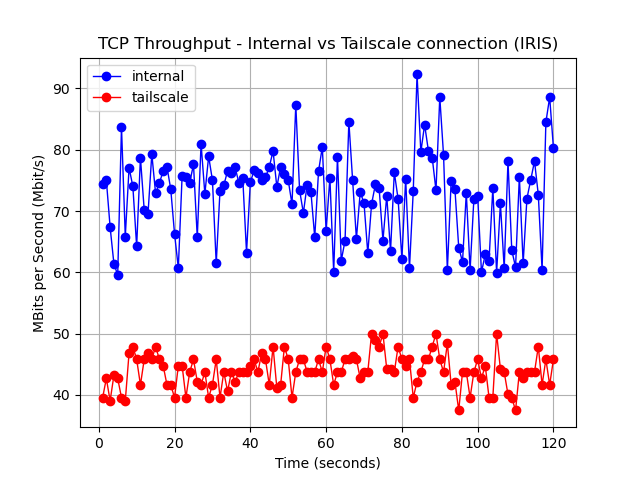
\includegraphics[width=0.9\textwidth]{overhead.png}
  \caption{Tailscale's toll on throughput, tested on internal and Tailscale connections inside IRIS-Lab}
  \label{fig:overhead}
\end{figure}

\begin{figure}[h]
\centering
  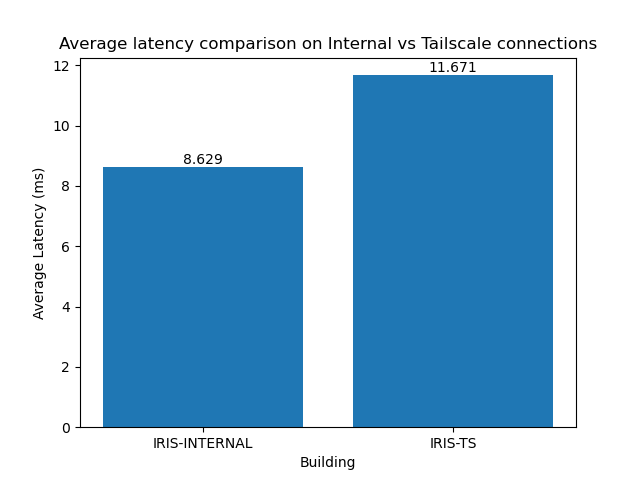
\includegraphics[width=0.8\textwidth]{latency_overhead.png}
  \caption{Round Trip Time distribution for internal (IRIS-I) and Tailscale (IRIS-TS) connections}
  \label{fig:latency_overhead}
\end{figure}


\section{Security and Confidentiality}

As we have seen, Tailscale encrypts and secures communications with WireGuard. This experiment aims to visualize how packets in the overlays are perceived by untrusted entities. A straightforward method to verify this dimension relies on the analysis of network captures. In fact, messages in a Tailscale tunnel can only be understood by the source and destination nodes. Traffic travelling through any other infrastructure is seen as an undecipherable stream of packets.

Hence, this validation operates by generating traffic between two overlay nodes and simultaneously capturing the packets in the destination node's Tailscale interface and in another intermediary network link's interface. On relayed connections, which is the case in this scenario, this intermediary capture is done in the \ac{DERP} server's interface. We can verify the encryption taking place by correlating packets from both captures using their timestamps as reference.

\subsection{Capturing and Visualising Traffic}

To capture packets on a network interface, \textbf{tcpdump} \footnote{Tcpdump, \url{https://www.tcpdump.org/}}, an open source command-line tool, was used. With this tool, we can initiate a capture by using the \textbf{tcpdump} command and pointing to a desired interface. Results from a capture can be exported to a file, which then allows a user friendly visualisation using \textbf{Wireshark} \footnote{Wireshark, \url{https://www.wireshark.org/}}, also an open source tool. Wireshark facilitates analysing and correlating the captures.

\subsection{Generating Traffic}

For the scope of this experiment, a client server scenario was created using two overlay nodes. One of the nodes runs a simple \ac{http} server, listening on its Tailscale interface, while the other generates traffic by executing requests to this server using \textbf{curl} \footnote{cURL, \url{https://curl.se/}}. Both nodes are connected to \ac{ua}'s network, hence the Tailscale connection is relayed.

\subsection{Experiment}

Having defined how traffic is generated and captured, the experiment starts by initiating two captures, one on the \ac{http} server's Tailscale interface and one on the \ac{DERP} server's Wi-Fi interface. Traffic associated with the generated \ac{http} requests will travel through both these interfaces, as all Tailscale traffic requires relaying by the \ac{DERP} server before reaching its respective destination.

With the captures running, \ac{http} requests were done by the client node, using cURL. After closing the captures, two pcap files are generated, which are loaded in Wireshark and correlated manually by analysing the packets' timestamps.

\subsection{Results}

Figure \ref{fig:cipher} presents both captures side by side in Wireshark. By analysing these results, the \ac{http} request and response are encapsulated as a \ac{tcp} stream on the \ac{DERP} server capture, and its payload encrypted, while the corresponding packets in the client's \ac{http} server's interface capture shows the same request and response as plain-text. Hence, Tailscale is effectively encrypting tunnel traffic, as only communication end nodes are able to decrypt and understand the information being transmitted.

\begin{figure}[h]
\centering
  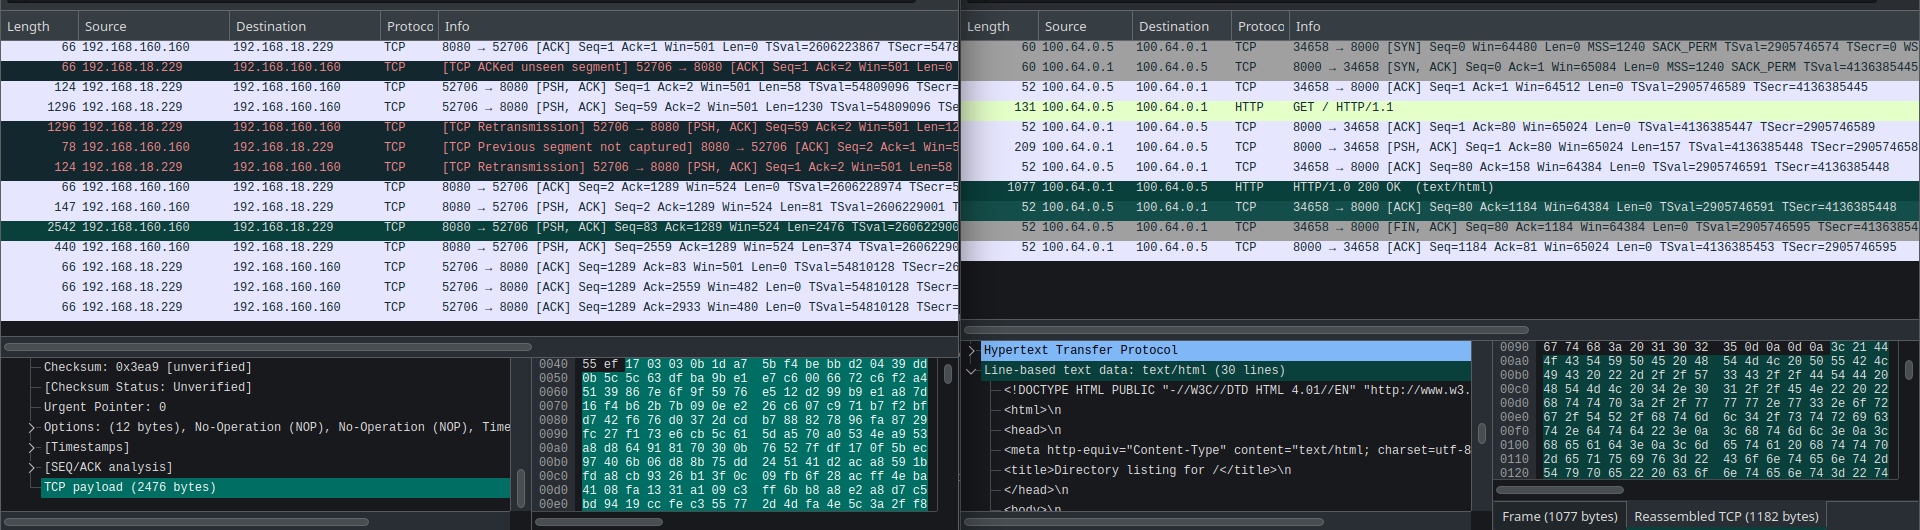
\includegraphics[width=0.9\textwidth]{cipher.png}
  \caption{TCP Streams from external capture (left) and destination node capture (right)}
  \label{fig:cipher}
\end{figure}

\section{Live Camera Feed Application}

The next experiment conducted aims to analyse how \ac{ros} applications operate when using the overlay networks. For that, a \ac{ros} application which publishes a camera feed is launched in a machine connected to \ac{iris}'s network. Then, in another \ac{ros} node, the output of the camera is accessed, from outside the laboratory, connected to the campus' network. With this experiment, we are able to compare metrics such as the video's bandwidth and framerate from the source against what a client actually consumes both when connected to the laboratory's internal network and when using the overlays.

\subsection{Camera and ROS Setup}

For this experiment, a two node \ac{ros} environment is created where the master node, running inside \ac{iris}'s network, publishes the feed from an external Astra camera to a topic. Then, another node subscribes this topic, being able to consume the camera feed.

Figure \ref{fig:camera} presents said setup.


\begin{figure}[h]
\centering
  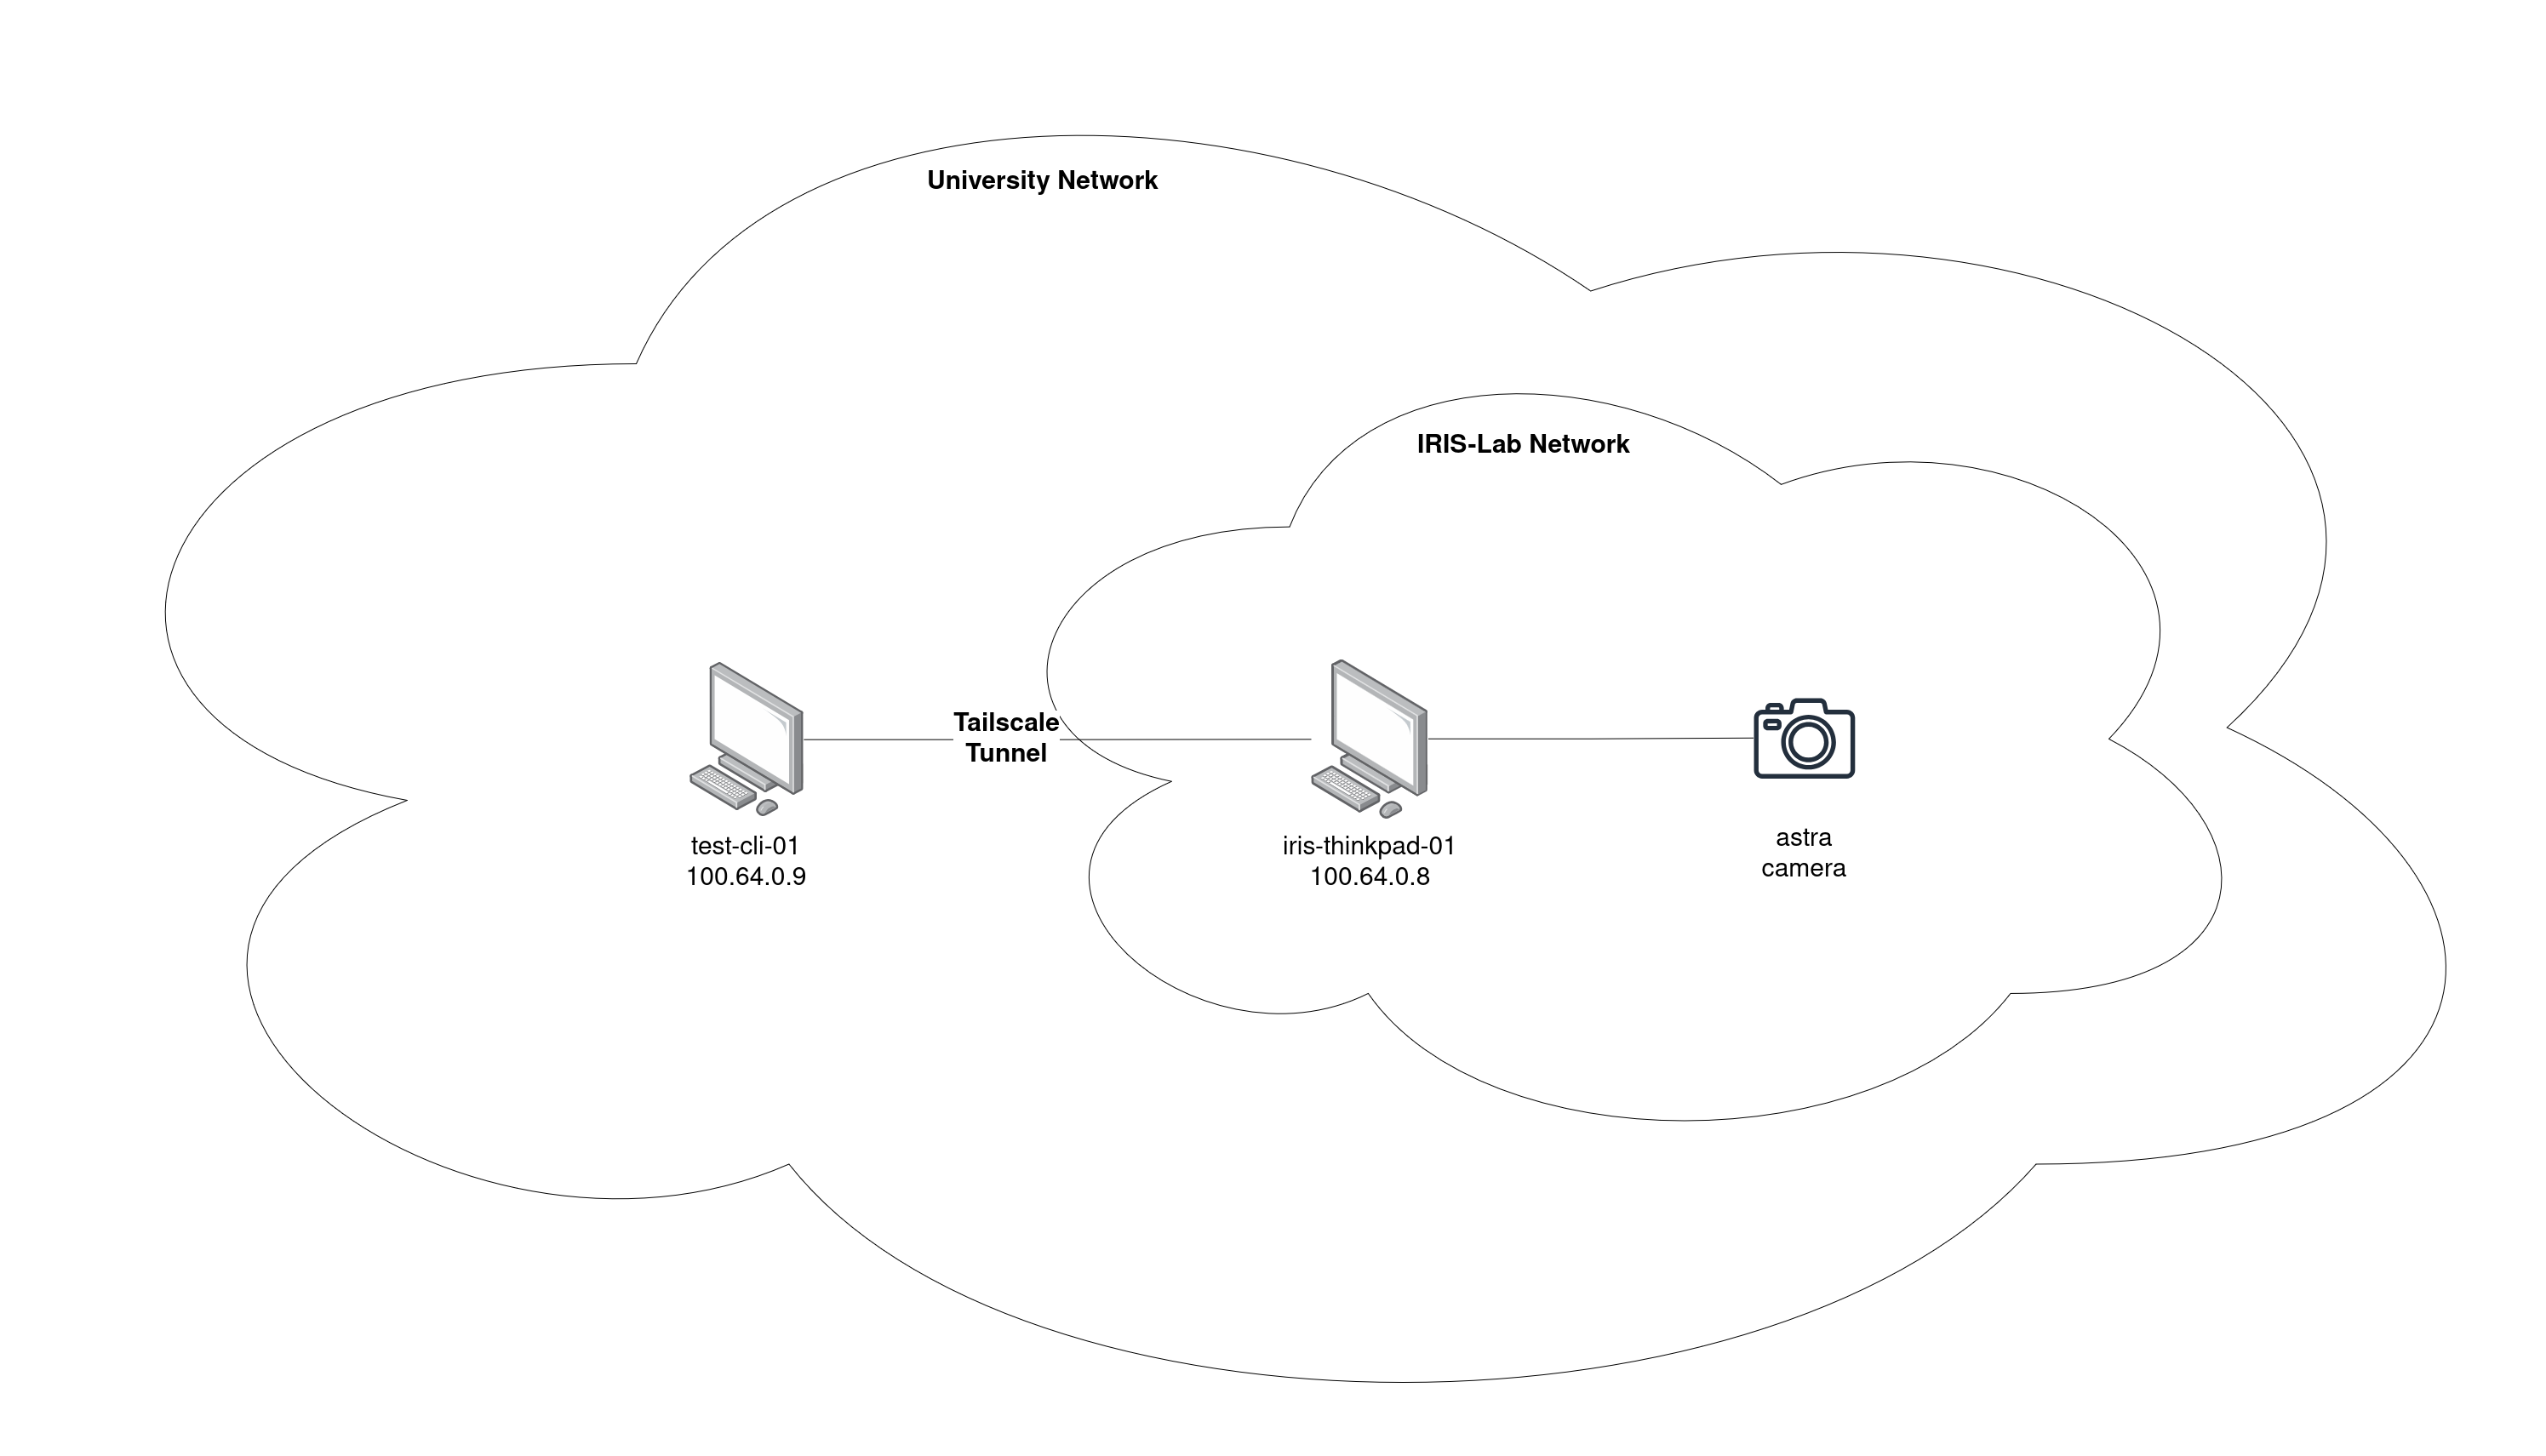
\includegraphics[width=\textwidth]{camera.png}
  \caption{Camera setup. The ROS node inside IRIS-lab's network publishes the camera feed.}
  \label{fig:camera}
\end{figure}

\subsection{Collecting Metrics}

The raw, uncompressed camera feed is published to the \textbf{$/$camera$/$color$/$image$_\_$raw} topic. Image bandwidth and frame rate can be calculated at both ends with the \textbf{rostopic bw} and \textbf{rostopic hz} commands. These two metrics are used to evaluate the solution's performance in this context.

Metrics were collected on two different scenarios. One with the consumer node also connected to \ac{iris}'s network and communicating through private \acp{ip} and one connected to \ac{ua}'s network, accessing the feed via Tailscale interfaces.

\subsection{Results}

Table \ref{tab:cam}.

\begin{table}[]
\centering
\begin{tabular}{c|c|c|c|}
\cline{2-4}
                                                                                                         & \textbf{\begin{tabular}[c]{@{}c@{}}Source Camera\\  Feed\end{tabular}} & \textbf{\begin{tabular}[c]{@{}c@{}}Internal \\  Consumer\end{tabular}} & \textbf{\begin{tabular}[c]{@{}c@{}}Tailscale \\ Consumer\end{tabular}} \\ \hline
\multicolumn{1}{|c|}{\textbf{\begin{tabular}[c]{@{}c@{}}Average Bandwidth\\ (MBytes / s)\end{tabular}}}  & 27.76                                                                  & 14.53                                                                             & 6.25                                                                              \\ \hline
\multicolumn{1}{|c|}{\textbf{\begin{tabular}[c]{@{}c@{}}Average Frame Rate\\ (frames / s)\end{tabular}}} & 30.060                                                                 & 14.582                                                                            & 6.515                                                                             \\ \hline
\end{tabular}
\caption{Streaming performance from source and consumer's end on internal and Tailscale connections}
\label{tab:cam}
\end{table}

\section{Robotic Arm Operation}

The last conducted experiment also aims to analyse the performance of \ac{ros} applications through the overlays. For this experiment, a robotic arm connected to a \ac{ros} Master residing in \ac{iris} is controlled by another \ac{ros} node, connected to \ac{ua}'s network.

\subsection{ROS Setup}

The robotic arm is directly connected to the master node and the \ac{ros} application is launched. Then, the slave node acknowledges the master node through its Tailscale \ac{ip}. The camera from the previous experiment is also setup, in order to have a visual feed of the robot movement when controlling it remotely. Figure \ref{fig:roboarm} presents this configuration.

\begin{figure}[h]
\centering
  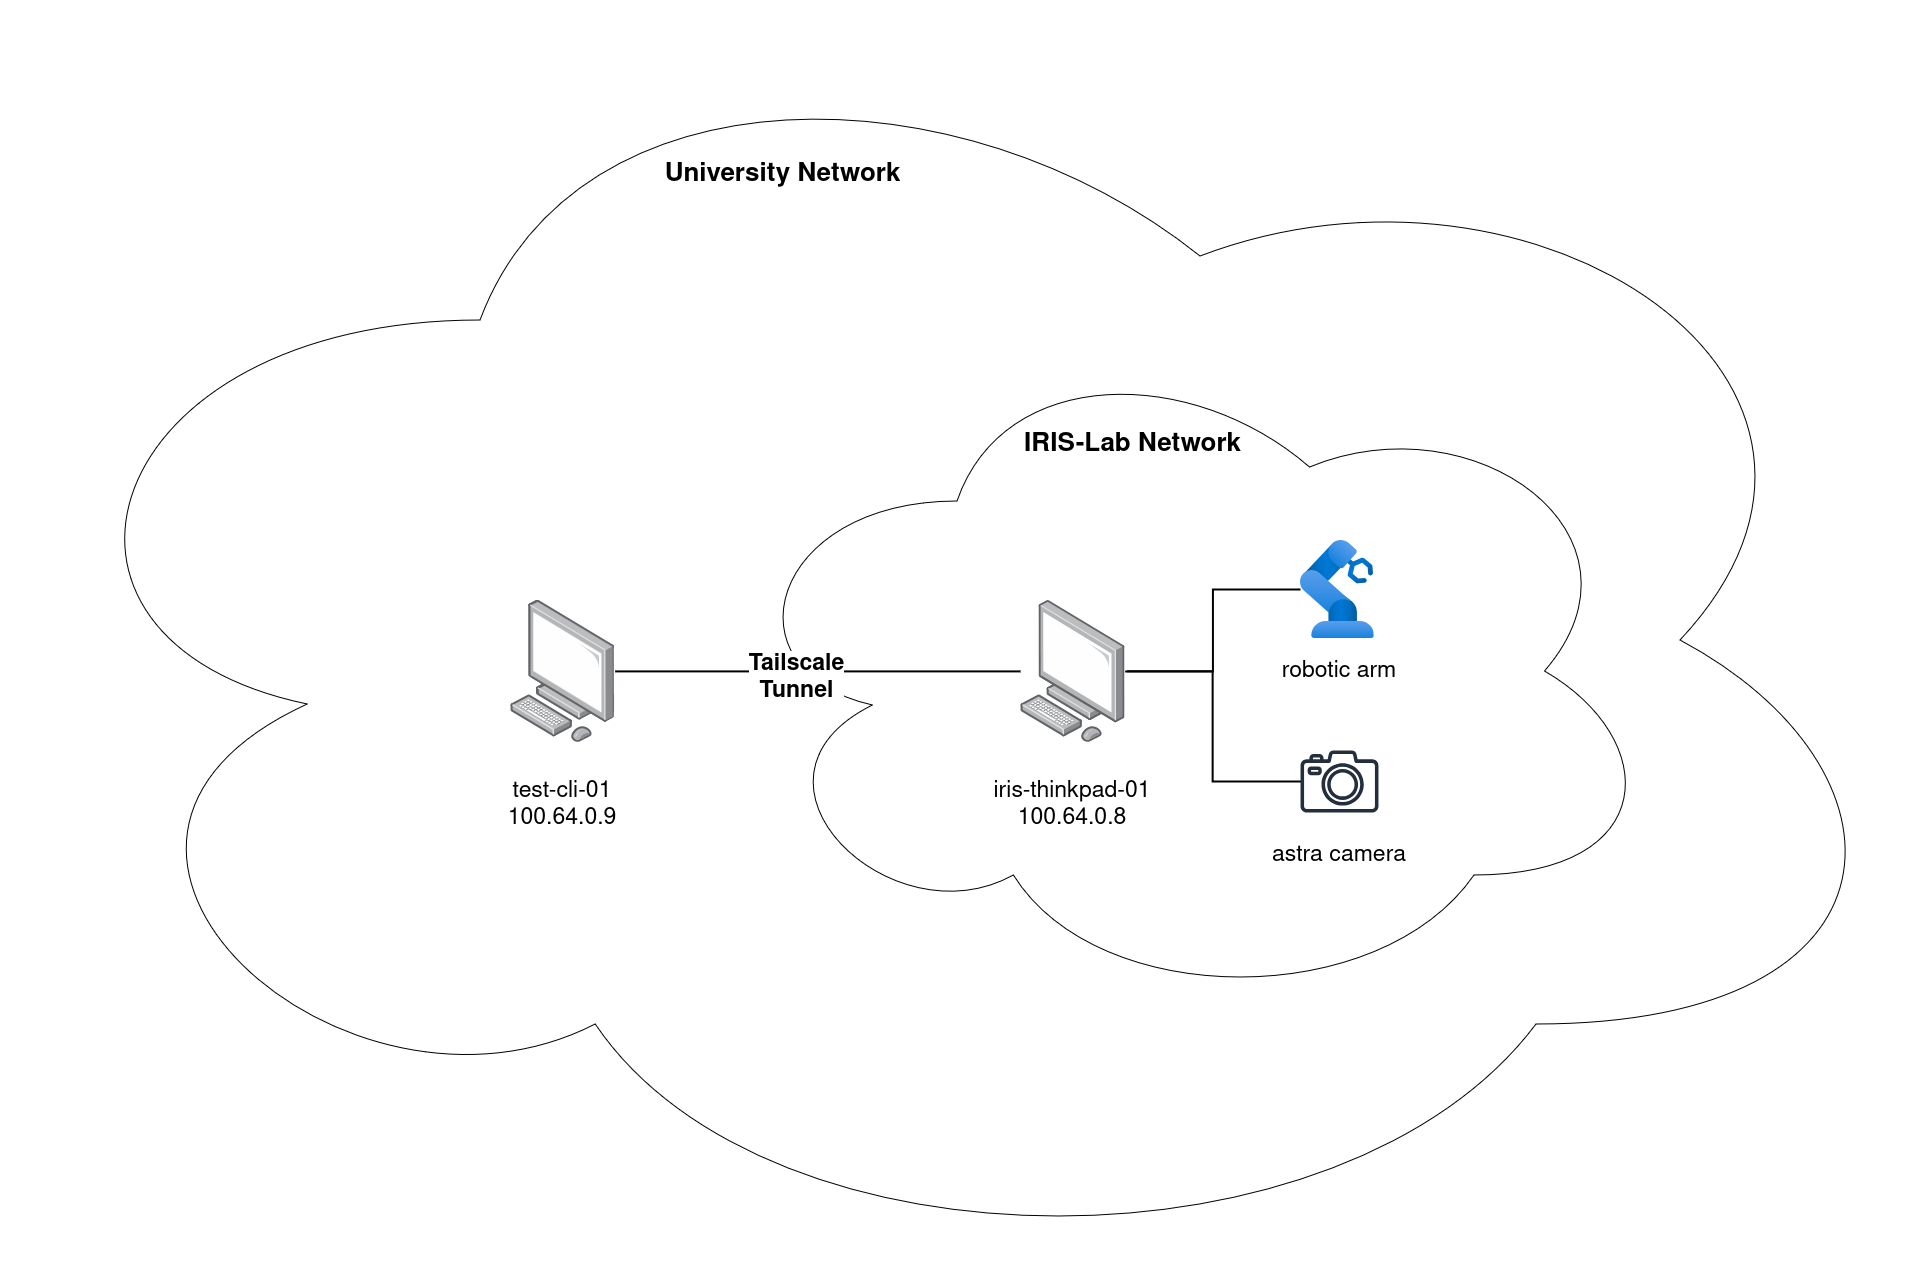
\includegraphics[width=\textwidth]{roboarm.png}
  \caption{Robotic Arm setup. The camera feed captures the robotic arm. The robot is operated through the ROS node residing in the University Network}
  \label{fig:roboarm}
\end{figure}

\subsection{Operating the Robotic Arm}

Moving the robot is achieved by maniuplating the robot's \textbf{joint\_states}, a \ac{ros} topic which contains the information regarding the arm's position.

To facilitate the operation of the robot, RViz \footnote{http://wiki.ros.org/rviz}, a 3D \ac{ros} visualization tool, was installed in the slave node. RViz provides an interface containing a 3D model of the robot, where movement can be planned by moving the joints on the model. Then, executing such a plan will generate and transmit the set of \ac{ros} messages responsible for updating the real robot's joints to match the position defined in the model.

Figure \ref{fig:armoperation} presents an example of operating the robot through RViz.

\begin{figure}[h!]
    \centering
    \begin{subfigure}[b]{0.45\textwidth}
        \centering
        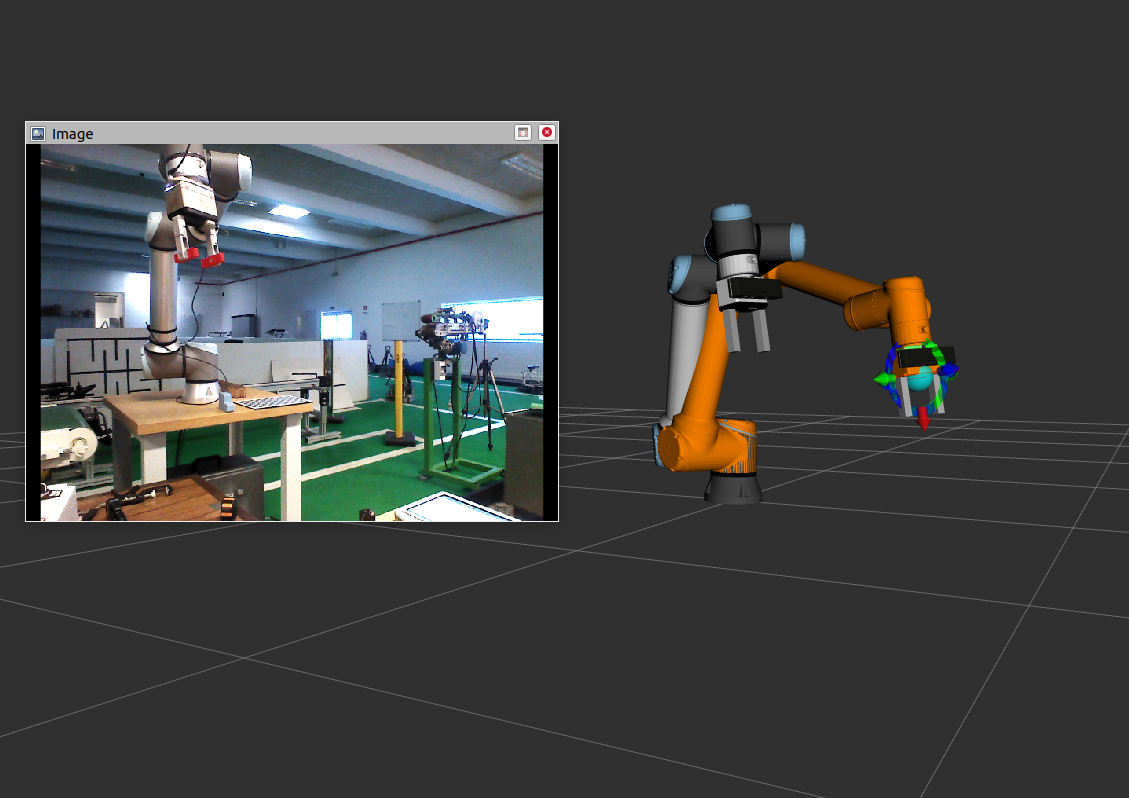
\includegraphics[width=\textwidth]{robot_initial.png}
        \caption{Robot's initial state. The orange outline represents the desired postion.}
        \label{fig:image1}
    \end{subfigure}
    \hfill
    \begin{subfigure}[b]{0.45\textwidth}
        \centering
        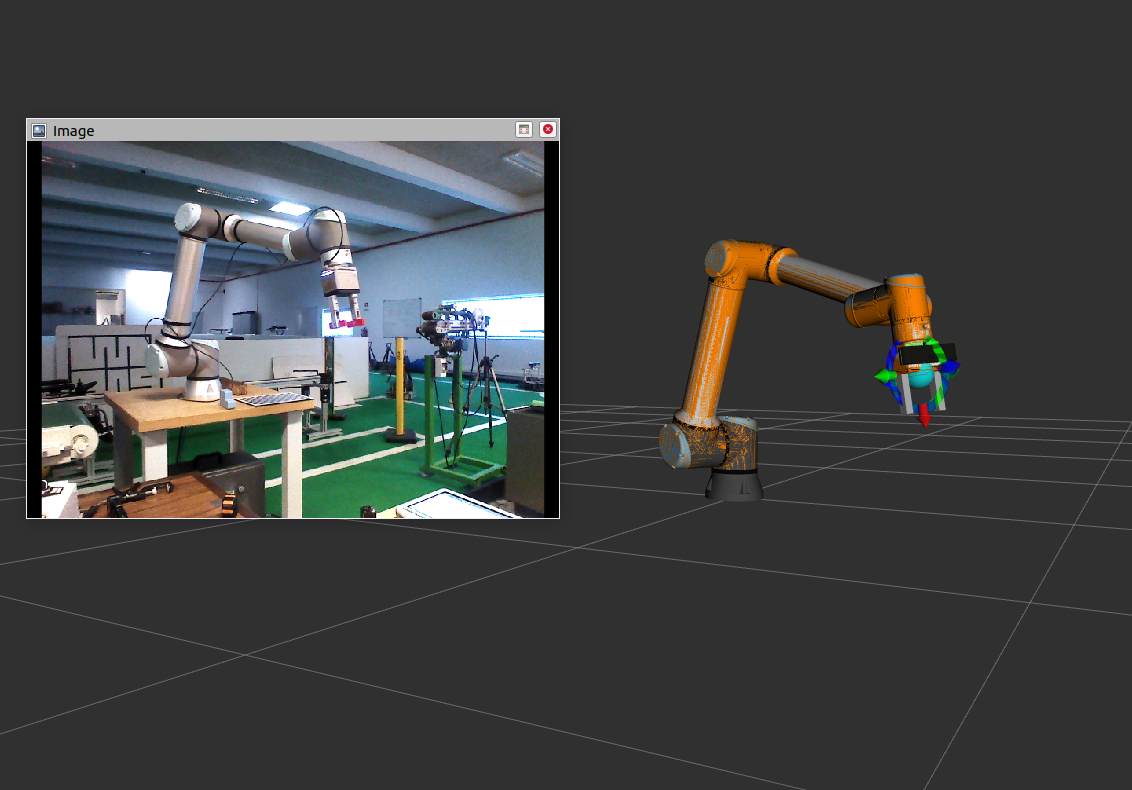
\includegraphics[width=\textwidth]{robot_final.png}
        \caption{Robot's state after executing the planned movement.}
        \label{fig:image2}
    \end{subfigure}
    \caption{Moving the robotic arm using RViz.}
    \label{fig:armoperation}
\end{figure}

\subsection{Results}

Operating the robot through the overlays performs very similarly to the usual robot operation, with no noticeable performance degradation. Since the messages involved in manipulating the robot's joints present an average bandwidth of around 148 KB/s, measured using the \textbf{rostopic bw} command, the loss of throughput associated with the overlays is negliable for this use case.

Due to safety precautions associated with unsupervised operation of the robot, this experiment was only conducted with the slave node (the one who plans and executes the movement) placed inside \ac{iris}, while connected to \ac{ua}'s network. However, a similar performance is expected from any other point in the campus, as suggested by the measured throughputs in experiment \ref{ss:netperf}.

\section{Chapter Summary}

This chapter presented how this solution was validated and its performance analysed. To collect network performance metrics, \textbf{iperf3} was used in a range of different scenarios. First, to gain insights on Tailscale's overhead, network tests were run in the same conditions, through regular interfaces and through Tailscale tunnel. The analysis of these two sets of values presented a loss of \textbf{46.23} \% in \ac{tcp} throughput and an increase in average latencies of \textbf{21.11} \% when using the overlays. Regarding camous coverage, which refers to the physical area the overlays can operate under, all identified key places were able to communicate via Tailscale relayed connections when connected to \ac{ua}'s network. Moreover, performance results from these experiments showed no particular anomalies, although, and as expected, certain areas overperform others.

Regarding the solution's suitability for \ac{iris}'s use cases, two \ac{ros} applications were analysed, where communication is done through Tailscale interfaces. First, a live camera streaming application, which published its uncompressed raw data, proved to be too demanding for the associated protocol overhead, resulting in a poor consumed food for real-time video standards. However, applications which require fewer network resources, such as the control of a robotic arm by updating its joint$_$states, operated smoothly, with no perceivable performance degradation.

\chapter{Conclusion and Future Work}

\section{Conclusion}

Concluding, this document presents the details for the implementation of a secure overlay network manager, hosted entirely in a private environment.

After a systematic review of general networking concepts and potential tools and services, WireGuard appeared as the most suitable protocol for encrypted communication.

Although creating stand alone WireGuard overlay networks is possible, it requires managing and configuring individual peers, a process raising scalability and ease of administration issues.

Fortunately, Tailscale addresses such flaws by offering a coordination server capable of orchestrating the creation and configuration of WireGuard peers and respective tunnels, without sacrificing WireGuard's state of the art performance. Additionally, Tailscale employs a set of mechanisms and infrastructure which are able to overcome network constraints that would normally prevent the direct establishment of a WireGuard connection.

To confine this solution to \ac{ua}'s network, Headscale, an open-source self-hosted implementation of Tailscale's coordination server, was used alongside necessary additional services, namely a \ac{DERP} and a \ac{stun} server. Regarding clients, these are required to trust Headscale's server certificate and run Tailscale's open source client software.

Regarding validation, network tests were run through the overlays, using \textbf{iperf3}. This allowed the measurement of Tailscale's protocol overhead on communication, which, as expected, resulted in a loss of throughput and increase in \ac{rtt}. These experiments also provide insights on the overall network performance across multiple campus areas. Finally, the solution was tested when applied to \ac{ros} applications, with successful results.

Overall, this project delivers automated procedures to configure and deploy a secure self-hosted overlay network manager requiring minimal client configuration, accomplishing the goals outlined in Section \ref{sec:obj}.

With \ac{iris}'s robots authenticated in the self-hosted Headscale control server and, consequently, configured with Tailscale interfaces, encrypted communication is possible from anywhere within \ac{ua}'s campus through \ac{http} relayed connections, successfully enabling robot operation outside \ac{iris}'s internal network.

The protocol's suitability for \ac{iris}'s applications was also studied. As expected, due to the losss of performance associated with relayed connections, applications with high network demand might prove unreliable  when used through the overlays

\section{Future Work}

Even though the developments presented in this document meet the goals as expected, serveral aspects of this solution could be improved or should be more thoroughly analysed.

First, regarding deployment automations, although the scripts presented in Chapter \ref{ch:auto} provide a configurable procedure to deploy both an Headscale server and Tailscale clients, this logic could easily be ported to more adequate \ac{iac} frameworks. In fact, the steps taken in said scripts are easily implemented as, for example, Ansible \footnote{Ansible, https://www.ansible.com/} playbooks. This would allow a team of robots to be defined as an Ansible inventory, creating a true one-touch deployment, not requiring the scripts to be run manually in each individual peer.

An \ac{acl} is a Tailscale functionality capable of adding an extra security layer to overlay networks by defining policies allowing or denying traffic between nodes. These policies can be applied to Tailscale users, tags, or client groups. Ideally, when deploying a team of robots, these should be grouped and traffic restricted to that specific group, creating an additional logical segmentation to the network, furthering the confidentiality and privacy of the solution.

Regarding implementation, such an \ac{acl} system could easily be built on top of the previous automation improvements. In other words, a one touch deployment of a team of robots through \ac{iac} software would allow the creation of Tailscale groups, associating a team's clients to that group and, finally, applying the \ac{acl}.

In Chapter \ref{chap:results}, the network tests were run for a duration of 15 minutes each. Evidently, this provides only but a glimpse of the actual network behaviour. To create a more accurate perception of the impact Tailscale has on network throughout the campus, these experiments should be redone using a more ample time frame. This could be achieved either by tweaking the python test script parameters or by setting up monitoring tools such as Grafana \footnote{Grafana, https://grafana.com/} integrated with \textbf{iperf3}'s metric collections. Using such a monitoring platform would also provide dashboards to help visualize the overall results.

Finally, this solution's scalability should also be properly analysed, by collecting network metrics as more peers are added to the overlays. In fact, the solution's coordination server introduces a bottleneck, namely  the single \ac{DERP}. As connections outside \ac{iris} network are all relayed, a single \ac{DERP} might suffer a degree of resource overloading, as all traffic is being relayed by this service.

%
% The bibliography
%
\cleardoublepage

\bibliographystyle{ieeetr}
\bibliography{refs}
\cleardoublepage

\end{document}
